\documentclass[preprint,12pt]{elsarticle}
\usepackage[T1]{fontenc}
\usepackage[utf8]{inputenc}
\usepackage{amsmath,amssymb,amsthm}
\usepackage{booktabs,multirow,array}
\usepackage{graphicx}
\usepackage{xcolor}
\usepackage{pifont}
\usepackage{algorithm}
\usepackage[noend]{algpseudocode}
\usepackage{tikz}
\usetikzlibrary{positioning,arrows.meta}
\usepackage[hidelinks]{hyperref}
\usepackage[a4paper,margin=2.5cm]{geometry}

\newtheorem{proposition}{Proposition}
\newcommand{\cmark}{\ding{51}}
\newcommand{\xmark}{\ding{55}}
\newcommand{\pmark}{$\circ$}

\journal{Computers \& Security}

\begin{document}
\begin{frontmatter}

\title{SLIDE: label-free sliced-Wasserstein drift detection and budgeted adaptation for LLM-generated phishing in e-mail streams}

\author[mcbu]{Osman Can \c{C}etlenbik\corref{cor1}}
\ead{osman.cetlenbik@cbu.edu.tr}
\cortext[cor1]{Corresponding author.}
\affiliation[mcbu]{organization={Big Data Analytics Program, Department of Statistics, Manisa Technical Sciences Vocational School, Manisa Celal Bayar University},
            city={Manisa},
            postcode={45140},
            country={T\"urkiye}}

\begin{abstract}
Language models let attackers rewrite phishing cheaply. A gateway detector trained on a fixed partition meets each rewrite as an unannounced shift of the message distribution, while verified labels for the new campaign arrive late and cost analyst time. We ask whether a transformer detector can recognise such shifts without labels and recover its accuracy from a small purchased label budget. SLIDE represents each e-mail by a fine-tuned DistilRoBERTa embedding and four language-model surprisal statistics. Its two-gate drift test applies Holm-corrected Kolmogorov--Smirnov tests to 64 random projections plus the detector score and requires a sliced-Wasserstein effect size above a reference-calibrated threshold; an alarm buys 500 labels, and the head is then retrained with class-balanced replay under representation-space adversarial training. Evaluation is prequential on a 28{,}000-message public stream that moves from seven human corpora to two LLM corpora and a T5 paraphrase campaign, over ten realisations and against nine baselines. SLIDE reached a stream MCC of 0.898 with 2{,}000 labels. Fully supervised ADWIN retraining of the same head also reached 0.898, and online TF-IDF learning 0.905, each with 27{,}500 labels. All 40 segment changes raised an alarm within one batch, with no false alarm. The same 2{,}000 labels bought at random times gave 0.786, whereas an oracle that knows the boundaries gave 0.902. A 400-character benign prefix cut the recall of every transformer detector to at most 0.11. Sliced label-free testing thus times label purchases close to an oracle at 7.3\% of the label cost.
\end{abstract}

\begin{keyword}
Phishing detection \sep Large language models \sep Concept drift \sep Sliced Wasserstein distance \sep Adversarial robustness \sep Data streams
\end{keyword}


\end{frontmatter}

\section{Introduction}\label{sec:intro}

Phishing is still the most common initial-access vector. Its production cost has collapsed since instruction-tuned language models began to write fluent, personalised lures from a few lines of reconnaissance \cite{heiding2024,hazell2023}; in controlled studies, fully automated LLM spear-phishing matched or exceeded the click-through rates of expert-written messages \cite{heiding2026,bethany2025}, and generator--critic loops now rewrite a lure until machine defenders stop flagging it \cite{qi2025}. Two consequences matter for a detector deployed at an e-mail gateway. The attacker can change the surface form of a campaign at negligible cost, by switching the generating model or by paraphrasing a known lure; that change reaches the gateway as an unannounced shift of the message distribution, observed at full throughput, long before verified labels for the new campaign exist.

Transformer detectors are evaluated almost exclusively on fixed partitions. Fine-tuned DistilBERT and RoBERTa encoders report F1 scores close to 0.99 in that setting \cite{jamal2024,uddin2026,ibrahim2026,safran2025,cetlenbik2024roberta}, yet the last two years of evidence show that such figures do not transfer: LLM rephrasing of known phishing lowers the accuracy of commercial filters and ML detectors \cite{afane2024,thapa2025}, and changing the generating model between training and deployment costs 28 F1 points while the AUC stays above 0.96 \cite{gutierrez2026}. The ranking survives that change; the operating threshold does not. Template artefacts in generated corpora can also turn in-distribution scores into a ceiling effect rather than evidence of learned semantics \cite{cetlenbik2026}.

Prior work leaves the streaming case open. The studies that model generative-AI shift explicitly do so offline, on predefined partitions \cite{arharbi2026,eskandarian2026}; the drift literature offers label-free detectors for deep representations \cite{rabanser2019,greco2025,wan2024,feldhans2024} and mature adaptation loops for malware and intrusion telemetry \cite{pan2026,han2026,yang2025,mcfadden2026}, but none of them has been specified for e-mail streams in which labels arrive late and cost analyst time while the shift itself may be adversarial. This paper asks whether a transformer-based phishing detector can notice, without labels, that the message distribution has moved, and then recover its accuracy from a small purchased label budget while paraphrase campaigns drive the move. We answer with SLIDE, a sliced-Wasserstein drift-adaptive defence, and with a prequential protocol built entirely from public corpora.

The contributions are four.
\begin{enumerate}
\item \textbf{A streaming threat model for LLM-era phishing} (Section~\ref{sec:formulation}). It couples delayed, budgeted labels with virtual drift measured by $SW_1$ and KS statistics in representation space, and with evasion families whose budgets are measured rather than assumed. A five-segment public benchmark stream moves from human corpora of 1999--2008 to two independent LLM corpora before ending in a paraphrase campaign; every source is audited for template leakage.
\item \textbf{A label-free sliced two-gate drift test} (Section~\ref{sec:test}). Holm-corrected KS tests on random projections and on the detector score are combined with a sliced-Wasserstein effect-size gate calibrated on the reference window. Proposition~\ref{prop:fwer} proves family-wise false-alarm control; Proposition~\ref{prop:sw} states what an alarm certifies about the underlying shift.
\item \textbf{A label-on-alarm adaptation policy with a composite robust objective} (Sections~\ref{sec:loss} and~\ref{sec:policy}). The objective has four terms: class-weighted cross-entropy on the purchased window, class-balanced reservoir replay, an $\ell_2$ adversarial loss in representation space and a proximal penalty that limits each update. A Lipschitz margin certificate (Proposition~\ref{prop:cert}) and a time and memory analysis (Proposition~\ref{prop:cost}) accompany the objective.
\item \textbf{A statistically controlled empirical study} (Section~\ref{sec:results}). SLIDE is compared with nine baselines, from static detectors to fully supervised retraining, over ten stream realisations under Friedman/Nemenyi and Holm-corrected Wilcoxon tests. The study adds three equal-budget timing controls, a nine-variant ablation, a sensitivity analysis, a six-variant evasion stress test and component-level latency on commodity CPU hardware; all code is released.
\end{enumerate}
The remainder follows the order of these contributions, with the results in Section~\ref{sec:results} and their limits in Section~\ref{sec:discussion}.

\section{Related work}\label{sec:related}

\subsection{LLM-generated phishing and spear-phishing}
Language models lowered the cost of personalised lures. Heiding et al.\ compared GPT-4 lures with the rule-based V-Triad and with their combination in a 112-participant study, and found that the same models could also serve as zero-shot intent detectors \cite{heiding2024}; a follow-up automated the whole spear-phishing pipeline and measured a 54\% click-through rate for AI-automated messages against 12\% for a control group \cite{heiding2026}. Bethany et al.\ ran lateral-phishing campaigns against roughly 9{,}000 university staff, with LLM-written messages as effective as those of communication professionals \cite{bethany2025}. Hazell documented the economics of LLM spear-phishing against more than 600 parliamentarians \cite{hazell2023}. SpearBot pairs a jailbroken generator with LLM critics that rewrite each e-mail until machine defenders no longer flag it \cite{qi2025}.

Defensive studies remain mostly static. Greco et al.\ separated LLM-written from human-written phishing with lightweight interpretable classifiers \cite{greco2024} and Eze and Shamir reported high accuracy on a public AI-generated corpus \cite{eze2024}, while Opara et al.\ evaluated commercial filters together with stylometric detectors on GPT-4o lures \cite{opara2025}; prompted or quantised LLMs have been benchmarked as detectors \cite{zhang2025,thapa2025}, and Koide et al.\ obtained 99.70\% accuracy with prompted GPT-4 on headers and bodies \cite{koide2026}. Two findings recur across this work. LLM rewriting of known phishing degrades classical filters and ML detectors alike \cite{afane2024,thapa2025}; a change of generating model produces a threshold-level failure, with a cross-model F1 drop of 28.0 points at an AUC above 0.96 that Gutierrez et al.\ close only by recalibrating on a labelled slice of the target generator \cite{gutierrez2026}. A recent systematisation asks for evaluations that span generators and manipulation strategies instead of a single corpus \cite{chen2025sok}. None of these studies monitors a stream for the onset of the shift, and none bounds the label cost of reacting to it.

\subsection{Transformer detectors and adversarial evasion}
Fine-tuned BERT-family encoders dominate recent e-mail detection. IPSDM fine-tuned DistilBERT and RoBERTa for three-class phishing/spam/ham detection \cite{jamal2024}; Uddin et al.\ coupled DistilBERT with LIME and Transformers-Interpret explanations \cite{uddin2026}, Ibrahim and Elhafiz compared BERT with RoBERTa on Nazario and Enron \cite{ibrahim2026}, PhishingGNN added graph attention to DistilBERT features on CEAS-08 \cite{safran2025}, and our earlier RoBERTa study reached a similar ceiling on a static split \cite{cetlenbik2024roberta}. Such in-distribution scores deserve caution. Our TurkPhish~v2 audit showed that a template-composed corpus can admit a zero-learning lookup rule with 0.928 macro-F1, and that eight of ten detectors became statistically indistinguishable in distribution while diverging on out-of-topic data \cite{cetlenbik2026}.

Robustness studies attack these encoders from single characters up to rendered web pages. Sajad applied FGM adversarial training with stochastic character noise to DistilBERT \cite{sajad2025}; Kulal et al.\ defended classical models against four TextAttack recipes and LLM-generated lures through spelling correction \cite{kulal2025}, Kulkarni et al.\ generated adversarial phishing web pages that lowered the detection rates of visual and multimodal detectors \cite{kulkarni2025}, and Rivera Soto et al.\ inverted paraphrases to restore machine-text detectors with a 22\% average AUROC gain \cite{riverasoto2025}. The two closest works treat generative-AI shift explicitly. Eskandarian et al.\ distilled a MobileBERT teacher into a 4.5M-parameter attention BiLSTM and tested it on LLM paraphrases under cross-distribution protocols \cite{eskandarian2026}, while Arharbi and El Qadi studied DistilBERT detectors under generative-AI shift with an interpretability-driven abstention gate on 864 LLM-written e-mails \cite{arharbi2026}; both evaluate fixed train/test partitions and do not observe the shift as it arrives.

\subsection{Concept drift detection in security and in text streams}
Malware and intrusion detection hold the deepest drift literature. TRANSCENDENT rejects drifting samples through conformal evaluation \cite{barbero2022}; Chen et al.\ combined hierarchical contrastive learning with active labelling after measuring an F1 decline from 0.99 to 0.76 within six months without updates \cite{chen2023usenix}, and drift forensics traced most such degradation to the rise of two families \cite{chow2023}. DriftTrace \cite{pan2026} and Argus \cite{han2026} detect and explain drift from contrastive representations before adapting to it. ReCDA adapts intrusion detectors from few labels \cite{yang2025}, and DRMD learns jointly to classify and to reject samples for labelling under a budget \cite{mcfadden2026}; on malware features, MMD-triggered retraining matched periodic retraining with far fewer updates \cite{berruz2026}. Sabbah et al.\ applied Kolmogorov--Smirnov tests to deprecated Android permissions \cite{sabbah2026} and measured how adversarial vulnerability grows with temporal distance \cite{sabbah2027}.

Generic label-free detectors operate on deep representations. Rabanser et al.\ found two-sample tests on reduced representations to be the most reliable shift detectors \cite{rabanser2019}; DriftLens computes distribution distances on embeddings in real time \cite{greco2025}, MCD-DD learns a maximum concept discrepancy \cite{wan2024} and ASK-NN proposes an asymmetric nearest-neighbour test for language representations \cite{zakharov2026}. For text, Feldhans et al.\ found multivariate kernel tests stronger than univariate KS tests on document embeddings, with lower dimensionality helping \cite{feldhans2021}, and later added per-sample drift scores and explanations \cite{feldhans2024}. Error-rate detectors such as DDM \cite{gama2004}, ADWIN \cite{bifet2007}, Page--Hinkley and KSWIN \cite{raab2020} remain the defaults of stream-learning libraries, and surveys formalise the distinction between real and virtual drift \cite{lu2019,hinder2024}. A recent preprint examines drift in ML phishing detectors \cite{fernando2026}. The e-mail literature still lacks a protocol in which delayed labels, label budgets, a generator change and an evasion campaign meet in one stream.

\subsection{Comparative matrix and positioning}
Table~\ref{tab:matrix} contrasts twelve 2024--2027 studies with SLIDE. Its columns follow the requirements of Section~\ref{sec:formulation}: drift handling, which asks whether shift is detected without labels and whether labels are delayed and budgeted, and adversarial evaluation against paraphrase or character-level evasion. Only one prior study receives full marks in both columns \cite{sabbah2027}, and it concerns Android malware rather than text; the e-mail studies with an adversarial column treat drift offline at best.

\begin{table*}[t]
\centering
\caption{Comparative matrix of recent work. D = drift handling, A = adversarial evaluation; \cmark\ yes, \pmark\ partial, \xmark\ no.}
\label{tab:matrix}
\scriptsize
\setlength{\tabcolsep}{3pt}
\begin{tabular}{@{}>{\raggedright\arraybackslash}p{3.5cm}>{\raggedright\arraybackslash}p{3.0cm}>{\raggedright\arraybackslash}p{2.6cm}cc>{\raggedright\arraybackslash}p{4.1cm}@{}}
\toprule
Study (venue, DOI) & Model & Data & D & A & Limitation addressed by SLIDE \\
\midrule
Afane et al.\ 2024, IEEE BigData \cite{afane2024} \newline{\tiny\url{10.1109/BigData62323.2024.10825018}} & Commercial filters, SVM/LR/NB, LLMs & Original vs.\ LLM-rephrased phishing & \pmark & \cmark & Measures the degradation; proposes no monitor or adaptation \\
Jamal et al.\ 2024, Secur.\ Priv.\ \cite{jamal2024} \newline{\tiny\url{10.1002/spy2.402}} & DistilBERT, RoBERTa (IPSDM) & Phishing/spam/ham sets & \xmark & \xmark & Static split; no LLM or evasion test \\
Thapa et al.\ 2025, SNPD \cite{thapa2025} \newline{\tiny\url{10.1109/SNPD65828.2025.11253009}} & Classical ML/DL vs.\ quantised LLMs & Curated static set & \xmark & \cmark & LLM inference cost; no shift detection \\
Safran \& Musleh 2025, IEEE Access \cite{safran2025} \newline{\tiny\url{10.1109/ACCESS.2025.3592135}} & DistilBERT + GAT & CEAS-08, Nazario & \pmark & \xmark & Cross-dataset only; no LLM lures \\
Greco et al.\ 2025, IEEE TKDE \cite{greco2025} \newline{\tiny\url{10.1109/TKDE.2025.3593123}} & DriftLens, embedding distances & Generic deep-learning streams & \cmark & \xmark & Not security-specific; no adaptation policy or label budget \\
Uddin et al.\ 2026, Comput.\ Netw.\ \cite{uddin2026} \newline{\tiny\url{10.1016/j.comnet.2026.112061}} & DistilBERT + LIME & Phishing e-mail corpus & \xmark & \xmark & Random split; no drift or robustness \\
Gutierrez et al.\ 2026, Front.\ Big Data \cite{gutierrez2026} \newline{\tiny\url{10.3389/fdata.2026.1883452}} & Stylometry + LR/XGBoost & 9{,}986 e-mails, 3 generators & \pmark & \xmark & Recalibration needs labelled target data \\
Eskandarian et al.\ 2026, JISA \cite{eskandarian2026} \newline{\tiny\url{10.1016/j.jisa.2026.104552}} & Distilled attention BiLSTM & Human + LLM paraphrases & \pmark & \cmark & Fixed partitions; no online detection \\
Arharbi \& El Qadi 2026, C\&S \cite{arharbi2026} \newline{\tiny\url{10.1016/j.cose.2026.105109}} & DistilBERT + SHAP/entropy gate & 864 LLM e-mails, 4 generators & \pmark & \cmark & Shift treated offline; no stream, delayed labels or label cost \\
Pan et al.\ 2026, IEEE TIFS \cite{pan2026} \newline{\tiny\url{10.1109/TIFS.2026.3659398}} & Contrastive AE (DriftTrace) & Drebin, MalDroid, IDS2018 & \cmark & \xmark & Tabular malware/IDS features, not text \\
Sabbah et al.\ 2027, ESWA \cite{sabbah2027} \newline{\tiny\url{10.1016/j.eswa.2026.133560}} & Multiple classifiers, FGSM/SPSA & Android, yearly slices & \cmark & \cmark & Not text; retraining assumes full labels \\
Feldhans \& Hammer 2024, IDEAL \cite{feldhans2024} \newline{\tiny\url{10.1007/978-3-031-77731-8\_28}} & Statistics on text embeddings & Text corpora & \cmark & \xmark & No security threat model, no adaptation \\
\midrule
\textbf{SLIDE (this work)} & DistilRoBERTa + LM surprisal + robust head & 7 human corpora, 2 LLM corpora, paraphrase campaign & \cmark & \cmark & Label-free sliced tests, label-on-alarm adaptation, measured label cost \\
\bottomrule
\end{tabular}
\end{table*}

\section{Problem formulation and threat model}\label{sec:formulation}

\subsection{Stream, labels and representation}
Let $\mathcal{X}$ be the space of e-mail strings (subject line followed by body) and $\mathcal{Y}=\{0,1\}$ with $y=1$ for malicious messages. The gateway observes a stream $\mathcal{S}=\{(x_i,y_i)\}_{i\ge 1}$ in batches $B_t=\{x_i : i\in I_t\}$ of size $b$, drawn from time-indexed joint distributions $P_t(X,Y)$. Scores must be produced for $B_t$ before any of its labels are known (prequential, test-then-train). A label $y_i$ for $i\in I_t$ can be obtained only at batch $t+D$ ($D\ge 1$ is the verification delay) and only if the operator purchases it, at unit cost. A detector is a pair $(f_t,\pi)$ of a scoring function $f_t:\mathcal{X}\to[0,1]$ and a labelling policy $\pi$ that decides which labels to buy. The total label cost after $T$ batches is $C_T(\pi)=\sum_{t\le T}|\pi(t)|$.

Every e-mail is mapped once to a representation $z=\Phi(x)\in\mathbb{R}^{d}$,
\begin{equation}
\Phi(x)=\big[\,\Sigma_\phi^{-1/2}(\phi(x)-\mu_\phi)\;;\;\Sigma_\psi^{-1/2}(\psi(x)-\mu_\psi)\,\big],\qquad d=d_\phi+d_\psi ,
\label{eq:phi}
\end{equation}
where $\phi(x)\in\mathbb{R}^{768}$ is the attention-masked mean of the last hidden layer of a DistilRoBERTa encoder fine-tuned on a warm-up window, $\psi(x)\in\mathbb{R}^{4}$ collects the mean, standard deviation, 10th and 90th percentiles of the token surprisal $-\log p_{\mathrm{LM}}(x_k\mid x_{<k})$ under a frozen causal language model, and the diagonal standardisation $(\mu,\Sigma)$ is estimated on the warm-up window only. Both $\phi$ and $\psi$ read the first $L=128$ sub-word tokens. A detection head $h_\theta:\mathbb{R}^d\to\mathbb{R}^2$ produces logits and $f_t(x)=\mathrm{softmax}(h_{\theta_t}(\Phi(x)))_1$; the decision rule is $\hat y=\mathbb{1}[f_t(x)\ge 0.5]$.

\subsection{Drift}
Write $P_t(X,Y)=P_t(X)\,P_t(Y\mid X)$ and let $Q_t=\Phi_\#P_t(X)$ denote the push-forward of the input marginal onto the representation space. Following the standard taxonomy \cite{lu2019,hinder2024}, \emph{virtual} drift between times $s<t$ is $Q_s\neq Q_t$ with $P_s(Y\mid X)=P_t(Y\mid X)$, and \emph{real} drift is a change of the posterior. A change of the generating mechanism of phishing (a new LLM or a paraphrased campaign) moves $Q_t$, and a detector trained on $Q_s$ is exposed to it whenever $h_{\theta_s}$ has not seen the new region. We quantify the movement with the order-1 Wasserstein distance
\begin{equation}
W_1(Q_s,Q_t)=\inf_{\gamma\in\Gamma(Q_s,Q_t)}\int\lVert z-z'\rVert_2\,\mathrm{d}\gamma(z,z'),
\end{equation}
and with its sliced version over the unit sphere $\mathbb{S}^{d-1}$,
\begin{equation}
SW_1(Q_s,Q_t)=\int_{\mathbb{S}^{d-1}}W_1\big(\theta_\#Q_s,\theta_\#Q_t\big)\,\mathrm{d}\sigma(\theta),\qquad \theta_\#Q(A)=Q(\{z:\langle\theta,z\rangle\in A\}),
\label{eq:sw}
\end{equation}
estimated with $K$ directions $\theta_1,\dots,\theta_K\overset{\mathrm{iid}}{\sim}\sigma$ \cite{kolouri2016}. On each one-dimensional projection the two-sample Kolmogorov--Smirnov statistic is $D_k=\sup_u|\hat F^{R}_{k}(u)-\hat F^{W}_{k}(u)|$, where $\hat F^{R}_{k}$ and $\hat F^{W}_{k}$ are the empirical CDFs of $\langle\theta_k,z\rangle$ on a reference sample $R$ and a test window $W$.

\paragraph{Drift hypotheses} For a reference sample $R\sim Q_s^{\otimes n_R}$ and a test window $W\sim Q_t^{\otimes n_W}$ we test
\begin{equation}
H_0:\;Q_s=Q_t\qquad\text{versus}\qquad H_1:\;SW_1(Q_s,Q_t)>\tau ,
\end{equation}
at family-wise level $\alpha$. The composite alternative contains an effect-size margin $\tau$ because, at e-mail-gateway volumes, a pure significance test rejects for operationally irrelevant differences \cite{demsar2006}.

\subsection{Threat model}\label{sec:threat}
The adversary controls the content of malicious messages but neither the gateway with its detector nor the labelling process (no poisoning). The adversary knows that a transformer-based filter is deployed and may query a generative model. We consider transformation families $\mathcal{T}$ applied to a phishing message $x$ with intent $\iota(x)$ and payload (URLs, addresses) preserved:
\begin{itemize}
\item[T1] \emph{Neural paraphrase.} Every payload-free sentence in the first $600$ characters is rewritten by a sequence-to-sequence paraphraser. The attacker accepts a rewrite $x'$ only if $\cos\big(e(x),e(x')\big)\ge 1-\epsilon_{\mathrm{sem}}$ with $\epsilon_{\mathrm{sem}}=0.30$ for an independent sentence encoder $e$ (MiniLM), and re-samples up to three times otherwise.
\item[T2] \emph{Character perturbation.} A fraction $\epsilon_{\mathrm{char}}\in\{0.05,0.10,0.20\}$ of eligible words (length $\ge 4$, payload excluded) receives a Cyrillic homoglyph or a zero-width space, or has two adjacent letters swapped.
\item[T3] \emph{Benign padding.} A 400-character fragment of a legitimate e-mail is prepended. The prefix pushes the lure towards the end of the $L$-token window that $\phi$ and $\psi$ read, or beyond it.
\end{itemize}
In the representation space the attacker's effective budget is $\epsilon_\Phi(x')=\lVert\Phi(x')-\Phi(x)\rVert_2$, which we report empirically rather than assume. The streaming campaign (segment~E, Section~\ref{sec:setup}) uses T1; the stress test uses T1--T3 and the composition T1$\circ$T2. The defender's objective is
\begin{equation}
\max_{f,\pi}\;\mathbb{E}\Big[\mathrm{MCC}\big(\{y_i\},\{\mathbb{1}[f_{t(i)}(x_i)\ge .5]\}\big)\Big]\quad\text{s.t.}\quad C_T(\pi)\le \beta T b ,
\label{eq:objective}
\end{equation}
that is, high prequential Matthews correlation under a label budget $\beta$ (fraction of the stream).

\section{The SLIDE framework}\label{sec:method}

SLIDE (\emph{Sliced-Wasserstein, Label-budgeted, Drift-adaptive Embedding defence}) has four components (Fig.~\ref{fig:arch}): (i) the hybrid representation $\Phi$ of Eq.~\eqref{eq:phi}; (ii) a robust detection head $h_\theta$ trained with the composite objective of Section~\ref{sec:loss}; (iii) a label-free sliced two-gate drift test on $\Phi$ (Section~\ref{sec:test}); and (iv) a label-on-alarm adaptation policy with a class-balanced replay memory (Section~\ref{sec:policy}). The encoder is fine-tuned once on the warm-up window and then frozen, so the per-message cost of the stream is one encoder pass and one causal-LM pass; everything that adapts operates on $d=772$-dimensional vectors.

\begin{figure}[t]
\centering
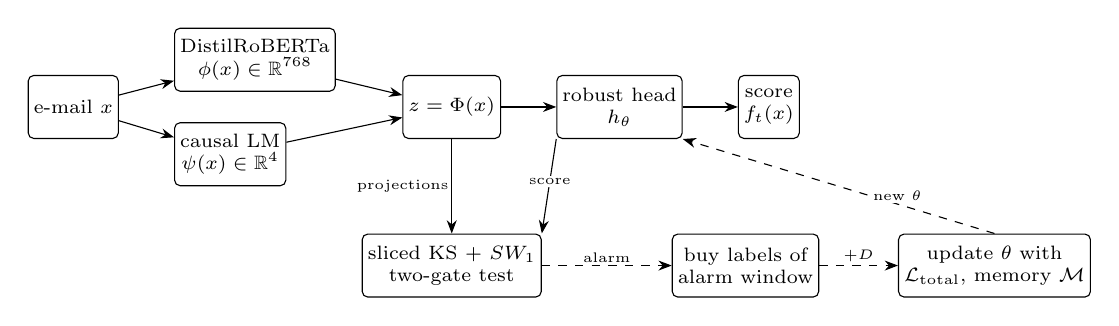
\begin{tikzpicture}[node distance=5mm and 7mm, every node/.style={font=\scriptsize}, box/.style={draw, rounded corners=2pt, align=center, minimum height=8mm, inner sep=2pt}, lab/.style={font=\tiny, fill=white, inner sep=1pt}, >=Stealth]
\node[box] (x) {e-mail $x$};
\node[box, right=of x, yshift=6mm] (enc) {DistilRoBERTa\\ $\phi(x)\in\mathbb{R}^{768}$};
\node[box, right=of x, yshift=-6mm] (lm) {causal LM\\ $\psi(x)\in\mathbb{R}^{4}$};
\node[box, right=10mm of x, xshift=26mm] (z) {$z=\Phi(x)$};
\node[box, right=of z] (h) {robust head\\ $h_\theta$};
\node[box, right=of h] (s) {score\\ $f_t(x)$};
\node[box, below=12mm of z] (t) {sliced KS + $SW_1$\\ two-gate test};
\node[box, below=12mm of h, xshift=16mm] (p) {buy labels of\\ alarm window};
\node[box, right=10mm of p] (u) {update $\theta$ with\\ $\mathcal{L}_{\mathrm{total}}$, memory $\mathcal{M}$};
\draw[->] (x) -- (enc); \draw[->] (x) -- (lm); \draw[->] (enc) -- (z); \draw[->] (lm) -- (z);
\draw[->] (z) -- (h); \draw[->] (h) -- (s); \draw[->] (z) -- node[lab, left]{projections} (t);
\draw[->] (h.south west) -- node[lab, pos=0.45]{score} (t.north east);
\draw[->, dashed] (t) -- node[lab, above]{alarm} (p);
\draw[->, dashed] (p) -- node[lab, above]{$+D$} (u);
\draw[->, dashed] (u.north) -- node[lab, right, pos=0.4]{new $\theta$} (h.south east);
\end{tikzpicture}
\caption{SLIDE data flow. Solid arrows run for every batch; dashed arrows run only after an alarm, when the labels of the alarm window are bought and arrive $D$ batches later.}
\label{fig:arch}
\end{figure}

\subsection{Robust head and composite objective}\label{sec:loss}
The head is a two-layer perceptron $h_\theta(z)=W_2\,\mathrm{GELU}(W_1z+c_1)+c_2$ with $W_1\in\mathbb{R}^{256\times d}$, dropout $0.1$ and $W_2\in\mathbb{R}^{2\times256}$. Given a newly labelled window $\mathcal{S}$ and a replay memory $\mathcal{M}$, with $\theta^{-}$ the parameters in force before the update, SLIDE minimises
\begin{equation}
\mathcal{L}_{\mathrm{total}}(\theta)=\underbrace{\mathcal{L}_{\mathrm{cls}}(\theta;\mathcal{S})}_{\text{new concept}}+\lambda_r\underbrace{\mathcal{L}_{\mathrm{cls}}(\theta;\mathcal{M})}_{\text{retention}}+\lambda_a\underbrace{\mathcal{L}_{\mathrm{adv}}(\theta;\mathcal{S}\cup\mathcal{M},\epsilon)}_{\text{robustness}}+\lambda_p\underbrace{\lVert\theta-\theta^{-}\rVert_2^2}_{\text{stability}},
\label{eq:ltotal}
\end{equation}
with the class-weighted cross-entropy
\begin{equation}
\mathcal{L}_{\mathrm{cls}}(\theta;\mathcal{A})=-\frac{1}{|\mathcal{A}|}\sum_{(z,y)\in\mathcal{A}}\omega_y\log\mathrm{softmax}\big(h_\theta(z)\big)_y,\qquad \omega_y=\frac{|\mathcal{S}\cup\mathcal{M}|}{2\,|\{(z',y')\in\mathcal{S}\cup\mathcal{M}:y'=y\}|},
\end{equation}
and the representation-space adversarial term
\begin{equation}
\mathcal{L}_{\mathrm{adv}}(\theta;\mathcal{A},\epsilon)=\frac{1}{|\mathcal{A}|}\sum_{(z,y)\in\mathcal{A}}\max_{\lVert\delta\rVert_2\le\epsilon}\;-\omega_y\log\mathrm{softmax}\big(h_\theta(z+\delta)\big)_y .
\label{eq:ladv}
\end{equation}
The inner maximisation is approximated by $P=3$ steps of normalised projected gradient ascent,
\begin{equation}
\delta^{(k+1)}=\Pi_{\mathbb{B}_\epsilon}\!\Big(\delta^{(k)}+\eta\,\frac{\nabla_\delta\ell(h_\theta(z+\delta^{(k)}),y)}{\lVert\nabla_\delta\ell(h_\theta(z+\delta^{(k)}),y)\rVert_2}\Big),\qquad \eta=\tfrac{2.5\,\epsilon}{P},\;\delta^{(0)}=0,
\end{equation}
where $\Pi_{\mathbb{B}_\epsilon}$ rescales onto the $\ell_2$ ball. Because $\Phi$ is standardised coordinate-wise, $\epsilon$ is expressed in units of warm-up standard deviations; $\lVert z\rVert_2\approx\sqrt{d}\approx 27.8$ for a typical message, so $\epsilon=1$ corresponds to a relative displacement of about 3.6\%. Real text attacks move $\Phi$ much further (Section~\ref{sec:stress}), which is why $\mathcal{L}_{\mathrm{adv}}$ is a smoothness regulariser for the head and not a defence on its own. The proximal term $\lambda_p\lVert\theta-\theta^-\rVert_2^2$ is an isotropic special case of elastic weight consolidation \cite{kirkpatrick2017}: it keeps the update in a neighbourhood of the previous solution while the replay term retains a class-balanced sample of earlier concepts. At initialisation ($\mathcal{S}$ = warm-up window, $\mathcal{M}=\emptyset$) the stability term is inactive. In every mini-batch the replay sample has the same size as the new-concept sample.

\paragraph{Margin certificate} Let $m_y(z)=h_\theta(z)_y-h_\theta(z)_{1-y}$. Because GELU is $\kappa$-Lipschitz with $\kappa\approx1.129$ and dropout is inactive at inference,
\begin{equation}
|m_y(z)-m_y(z')|\le L_m\lVert z-z'\rVert_2,\qquad L_m=\kappa\,\big\lVert (W_2)_{1,:}-(W_2)_{0,:}\big\rVert_2\,\lVert W_1\rVert_2 .
\label{eq:lip}
\end{equation}
\begin{proposition}[Certified invariance]\label{prop:cert}
If $m_y(z)>L_m\,\epsilon$, then $\arg\max h_\theta(z+\delta)=y$ for every $\lVert\delta\rVert_2\le\epsilon$.
\end{proposition}
\begin{proof}
By Eq.~\eqref{eq:lip}, $m_y(z+\delta)\ge m_y(z)-L_m\lVert\delta\rVert_2>L_m\epsilon-L_m\epsilon=0$.
\end{proof}
Proposition~\ref{prop:cert} is a sufficient condition and $L_m$ is a product bound, so the certified fraction it yields is conservative; we report it alongside empirical attack outcomes (Section~\ref{sec:stress}).

\subsection{Label-free sliced two-gate drift test}\label{sec:test}
SLIDE holds a reference matrix $R\in\mathbb{R}^{n_R\times d}$ of the first $n_R$ unlabelled stream representations scored by the current head (never the data it was fitted on), and a set $\Theta=[\theta_1,\dots,\theta_K]$ of random unit directions drawn once. The detector score $s(z)=f_t$ is appended as projection $K+1$ because it is the one-dimensional summary that the decision rule actually thresholds. After each batch the test window $W$ is formed from the last $n_W$ representations, and a test is run only once at least $n_W$ messages have arrived after $R$ was frozen, so that $W$ and $R$ never share a message. Two gates are evaluated.

\emph{KS gate.} For $j=1,\dots,K+1$ compute the asymptotic two-sample KS $p$-value $p_j$ of $D_j$. The gate fires if the Holm step-down procedure rejects at least one of the $K+1$ hypotheses at level $\alpha$, which is equivalent to $\min_j p_j\le \alpha/(K+1)$.

\emph{SW gate.} Compute $\widehat{SW}_1(R,W)=K^{-1}\sum_{k=1}^K W_1(\theta_{k\#}\hat R,\theta_{k\#}\hat W)$ with one-dimensional $W_1$ evaluated from sorted samples. The threshold $\tau_\alpha$ is the empirical $(1-\alpha)$ quantile of $\widehat{SW}_1(R_1,R_2)$ over $B=100$ random disjoint pairs $R_1,R_2\subset R$ with $|R_1|=|R_2|=\min(n_W,\lfloor n_R/2\rfloor)$. The gate fires if $\widehat{SW}_1(R,W)>\tau_\alpha$.

An alarm requires both gates. The KS gate controls the error rate; the SW gate imposes an effect-size margin calibrated on the reference itself, so that the detector does not react to statistically detectable but small fluctuations.

\begin{proposition}[False-alarm control]\label{prop:fwer}
Let the rows of $R$ and $W$ be independent draws from the same continuous distribution $Q$ and let $\Theta$ be drawn independently of $(R,W)$. Then, asymptotically in $n_R,n_W$, $\Pr(\text{alarm})\le\alpha$.
\end{proposition}
\begin{proof}
Conditionally on $\Theta$, each projected pair of samples is i.i.d.\ from the same continuous univariate law, so each $p_j$ is asymptotically super-uniform. Holm's procedure controls the family-wise error rate at $\alpha$ under arbitrary dependence among the $p_j$, hence $\Pr(\text{KS gate})\le\alpha$ conditionally on $\Theta$ and therefore unconditionally. The alarm is the conjunction of the KS gate with a second event, so $\Pr(\text{alarm})\le\Pr(\text{KS gate})\le\alpha$. The score projection $s(z)$ is a fixed measurable function of $z$ once the head is fitted on data disjoint from $W$, so the argument covers $j=K+1$.
\end{proof}
Proposition~\ref{prop:fwer} bounds the false-alarm probability of a single test. A stream runs about 80 tests, and consecutive windows overlap, so the per-stream false-alarm count is bounded in expectation by $80\alpha=0.8$ only through a union bound; Section~\ref{sec:boundaries} reports the observed count.

\begin{proposition}[Sliced distance as a certificate of shift]\label{prop:sw}
For any $Q,Q'$ with finite first moments, $SW_1(Q,Q')\le W_1(Q,Q')$, and $SW_1(Q,Q')=0$ if and only if $Q=Q'$. If the conditional expected loss $g(z)=\mathbb{E}[\ell(h_\theta(z),Y)\mid \Phi(X)=z]$ is $L_g$-Lipschitz and the posterior is unchanged (virtual drift), then $|\mathcal{R}_{Q'}(h_\theta)-\mathcal{R}_{Q}(h_\theta)|\le L_g\,W_1(Q,Q')$.
\end{proposition}
\begin{proof}
For fixed $\theta\in\mathbb{S}^{d-1}$ the map $z\mapsto\langle\theta,z\rangle$ is 1-Lipschitz, so for any coupling $\gamma$ of $(Q,Q')$ the image coupling of $(\theta_\#Q,\theta_\#Q')$ satisfies $\int|\langle\theta,z-z'\rangle|\,\mathrm{d}\gamma\le\int\lVert z-z'\rVert\,\mathrm{d}\gamma$; taking the infimum and averaging over $\theta$ gives the inequality. If $SW_1=0$ then $\theta_\#Q=\theta_\#Q'$ for $\sigma$-almost every $\theta$, and by continuity of characteristic functions for all $\theta$, so $Q=Q'$ by the Cram\'er--Wold theorem. The risk bound follows from Kantorovich--Rubinstein duality, $\big|\int g\,\mathrm{d}Q-\int g\,\mathrm{d}Q'\big|\le L_g W_1(Q,Q')$.
\end{proof}
Proposition~\ref{prop:sw} explains what an alarm certifies and what it does not. A large $\widehat{SW}_1$ is a lower bound on $W_1$ and therefore on the transport effort separating the two regimes, but a small $SW_1$ does not bound the risk change, and real drift with $Q_s=Q_t$ is invisible to any label-free test. Section~\ref{sec:validity} returns to this limitation.

\paragraph{Calibration remark} The empirical $W_1$ between two samples of sizes $(n,m)$ from the same law concentrates at a rate governed by $\sqrt{1/n+1/m}$. The null pairs used for $\tau_\alpha$ have sizes $(n_W,n_W)$ while the test compares sizes $(n_R,n_W)$ with $n_R=2n_W$, so the calibrated threshold is conservative.

\subsection{Label-on-alarm adaptation}\label{sec:policy}
When an alarm is raised at batch $t$, SLIDE purchases the labels of the last $\lceil n_\ell/b\rceil$ batches (the alarm window, $n_\ell=500$ messages), which all arrive at $t+D$; labels requested for a batch older than $t$ are therefore not received earlier than the others. Further tests are suspended until then. At $t+D$, as soon as the labels arrive, the head is updated with Eq.~\eqref{eq:ltotal}, warm-started from $\theta^-$, the labelled window is inserted into the memory, and the reference $R$ is rebuilt from the next $n_R$ representations scored by the new head, so that the next test compares post-adaptation data with post-adaptation data. The memory keeps at most $c=1000$ items per class by per-class reservoir sampling, which gives every labelled item seen so far the same inclusion probability. Algorithm~\ref{alg:slide} lists the procedure.

\begin{algorithm}[t]
\caption{SLIDE prequential detection with label-on-alarm adaptation}\label{alg:slide}
\small
\begin{algorithmic}[1]
\Require warm-up set $\mathcal{W}=\{(x_i,y_i)\}$, encoder $\phi$, LM $p_{\mathrm{LM}}$, $K,\alpha,B,n_R,n_W,n_\ell,c,D,\epsilon,\lambda_r,\lambda_a,\lambda_p$
\State fine-tune $\phi$ on $\mathcal{W}$; estimate $(\mu,\Sigma)$ on $\mathcal{W}$; $Z_{\mathcal{W}}\gets\Phi(\mathcal{W})$
\State $\theta\gets\arg\min\mathcal{L}_{\mathrm{total}}$ on $(\mathcal{S}{=}Z_{\mathcal{W}},\mathcal{M}{=}\emptyset)$ with $\lambda_p=0$; $\mathcal{M}\gets\textsc{Reservoir}(Z_{\mathcal{W}},c)$
\State draw $\Theta\in\mathbb{R}^{d\times K}$ with i.i.d.\ uniform unit columns; mark $R$ stale; $t_{\mathrm{ready}}\gets -\infty$
\For{$t=1,2,\dots$}
  \State $Z_t\gets\Phi(B_t)$; \textbf{emit} $f_t=\mathrm{softmax}(h_\theta(Z_t))_1$; append $Z_t$ to the buffer \Comment{test first}
  \If{$R$ stale}
    \If{$n_R$ rows are buffered} $R\gets$ last $n_R$ rows; $\tau_\alpha\gets\textsc{Calibrate}(R,B)$; $m\gets 0$ \EndIf
  \Else
    \State $m\gets m+b$
    \If{$m\ge n_W$ \textbf{and} $t>t_{\mathrm{ready}}$}
      \State $W\gets$ last $n_W$ rows; $p_j\gets\mathrm{KS}(\langle\theta_j,R\rangle,\langle\theta_j,W\rangle)$, $j\le K$; $p_{K+1}\gets\mathrm{KS}(s(R),s(W))$
      \If{$\min_j p_j\le\alpha/(K+1)$ \textbf{and} $\widehat{SW}_1(R,W)>\tau_\alpha$}
        \State request labels of batches $t-\lceil n_\ell/b\rceil+1,\dots,t$, due at $t+D$; $t_{\mathrm{ready}}\gets t+D$
      \EndIf
    \EndIf
  \EndIf
  \If{labels $\mathcal{S}$ are due at $t$}
    \State $\theta\gets\arg\min_\theta\mathcal{L}_{\mathrm{total}}(\theta;\mathcal{S},\mathcal{M},\theta^-{=}\theta)$ from $\theta^-$; $\mathcal{M}\gets\textsc{Reservoir}(\mathcal{M}\cup\mathcal{S},c)$; mark $R$ stale; clear the buffer
  \EndIf
\EndFor
\end{algorithmic}
\end{algorithm}

\subsection{Complexity}\label{sec:complexity}
Let $C_\phi$ and $C_\psi$ be the per-message costs of the encoder and LM passes ($\mathcal{O}(L^2 d_{\mathrm{model}}+L d_{\mathrm{model}}^2)$ per layer for a transformer with $L$ tokens), $h=256$ the hidden width and $n=n_R+n_W$.

\begin{proposition}[Per-batch cost]\label{prop:cost}
Scoring a batch costs $\mathcal{O}\big(b(C_\phi+C_\psi+dh)\big)$ time. One drift test costs $\mathcal{O}\big(n_W dK+Kn\log n\big)$ time, reducible to $\mathcal{O}(n_WdK+K n_W\log n_W+Kn)$ by keeping the projected reference sorted; calibration costs $\mathcal{O}(n_RdK+BKn_R\log n_R)$ once per reference. An update costs $\mathcal{O}\big(E\,(|\mathcal{S}|+\min(|\mathcal{S}|,|\mathcal{M}|))\,(P+1)\,dh\big)$ for $E$ epochs. The persistent state occupies $\mathcal{O}(dh+dK+Kn_R+cd)$ memory.
\end{proposition}
\begin{proof}
Projection of the window is a $(n_W\times d)(d\times K)$ product. For each of the $K+1$ projections the KS statistic and the one-dimensional $W_1$ are computed from the merged order statistics, which costs one sort of $n$ values, or a merge of a pre-sorted reference with a sorted window. Calibration repeats the $W_1$ computation $B$ times on reference subsets. In an update, each epoch visits every item of $\mathcal{S}$ once together with an equally sized replay sample, and each visit costs one forward and backward pass of the head plus $P$ PGD steps, each of which is another forward and backward pass. The state consists of $\theta$, $\Theta$, the projected and raw reference, and the memory.
\end{proof}
With $K=64$, $n_R=1000$, $n_W=500$ and $d=772$ the test does not depend on the batch size. Measured in isolation it takes 77\,ms per batch, or 0.31\,ms per e-mail, against 27\,ms per e-mail for the encoder pass on four threads (Section~\ref{sec:cost}); scoring cost is therefore dominated by $C_\phi+C_\psi$, and the drift machinery adds less than one percent to it.

\section{Experimental setup}\label{sec:setup}

\subsection{Corpora and stream construction}
All data are public. Human-written traffic comes from the unified release \cite{ds_seven} of the seven corpora curated by Champa et al.\ \cite{champa2024}: Enron and Ling-Spam with SpamAssassin (1999--2004), TREC-05/06/07 (2005--2007) and CEAS-08 (2008), 203{,}017 messages in total. Their positive class is the union of phishing and spam, which we refer to as \emph{malicious} and discuss in Section~\ref{sec:validity}. LLM-written traffic comes from two independent releases: \emph{GPTGen} \cite{ds_gptgen}, 3{,}746 English phishing and legitimate messages generated with OpenAI models, and \emph{SpearGen} \cite{ds_spear}, 2{,}798 personalised spear-phishing messages generated by an OpenAI model from a name, a job title and a list of recent activities. We remove inline sender addresses from GPTGen (they occur in no other corpus and would act as an artefact), normalise whitespace, prefix human messages with their subject line, discard human messages of 40 characters or fewer and SpearGen outputs of 80 characters or fewer and remove exact duplicates across all sources. Disjoint pools are then drawn with a fixed seed (Table~\ref{tab:pools}); no text appears in more than one pool.

\begin{table}[t]
\centering
\caption{Disjoint pools (legitimate/malicious counts). Each realisation samples its segments from these pools.}
\label{tab:pools}
\scriptsize
\setlength{\tabcolsep}{2.5pt}
\begin{tabular}{@{}lrr>{\raggedright\arraybackslash}p{9cm}@{}}
\toprule
Pool & Legit. & Malic. & Sources (legit./malic.) \\
\midrule
warm-up & 2295 & 1705 & Assassin 433/175; Enron 1605/1488; Ling 257/42 \\
segment A & 4649 & 3351 & Assassin 851/344; Enron 3301/2909; Ling 497/98 \\
segment B & 4474 & 3526 & TREC-05 2119/1455; TREC-06 781/256; TREC-07 1574/1815 \\
segment C & 3582 & 4418 & CEAS-08 3582/4418 \\
segment D & 4400 & 3300 & CEAS-08 607/0; GPTGen 900/1500; SpearGen 0/1800; TREC-05 1400/0; TREC-06 507/0; TREC-07 986/0 \\
segment E (orig.) & 2700 & 0 & CEAS-08 471/0; TREC-05 1036/0; TREC-06 380/0; TREC-07 813/0 \\
segment E (T1) & 300 & 1500 & CEAS-08 0/119; GPTGen 300/500; SpearGen 0/500; TREC-05 0/149; TREC-06 0/34; TREC-07 0/198 \\
stress pool & 0 & 600 & CEAS-08 0/51; GPTGen 0/200; SpearGen 0/200; TREC-05 0/62; TREC-06 0/13; TREC-07 0/74 \\
\bottomrule
\end{tabular}
\end{table}


Each stream realisation (seed $r=0,\dots,9$) samples, without replacement, the five segments in a fixed order, shuffling messages inside each segment: A (6{,}000 human messages, 1999--2004), B (6{,}000, TREC), C (6{,}000, CEAS-08), D (6{,}000: LLM phishing from GPTGen and SpearGen at 30\% prevalence, mixed with GPTGen legitimate messages and held-out human legitimate traffic) and E (4{,}000: a paraphrase-evasion campaign of 1{,}500 T1-attacked messages, about 1{,}250 of them malicious and drawn from the two LLM corpora and from human sources, the rest a paraphrased legitimate control, mixed with 2{,}500 human legitimate messages). Malicious prevalence is 42\%, 44\%, 55\%, 30\% and 31\% in A to E. Rewrites that stayed below the similarity budget after three tries are rejected and sent unmodified (3.4\% of attempts, about 45 messages per E segment). The boundaries A$\to$B$\to$C are natural temporal and source shifts; C$\to$D is a generator shift; D$\to$E is an adversarial shift. The stream is processed in $b=250$-message batches with label delay $D=2$ batches. The warm-up window (4{,}000 messages from the 1999--2004 corpora) is the only data used to fine-tune the encoder and to fit the standardisation; every initial detector is trained on it alone. A held-out stress pool of phishing messages from all three malicious sources is never streamed and is used only in Section~\ref{sec:stress}.

\subsection{Leakage and artefact audit}
Generated corpora can encode their label in templates rather than semantics \cite{cetlenbik2026}. Before any experiment we therefore audited every source$\times$class cell for template collapse after entity masking (URLs, addresses, numbers and capitalised spans), near-duplicates (pairwise TF-IDF cosine on up to 1{,}500 sampled messages), length balance, a zero-learning opening-trigram lookup rule, and a human-versus-LLM authorship probe on legitimate mail. The results (Section~\ref{sec:audit}) shape the evaluation: SLIDE and all baselines are scored separately on LLM-written legitimate messages so that a detector that learns ``LLM style'' instead of ``malicious intent'' is exposed by its false-positive rate.

\subsection{Compared methods}
Table~\ref{tab:methods} lists the ten methods, grouped by the supervision they consume. Static detectors never see stream labels; the fully supervised adaptive detectors receive every label after the delay $D$, whereas label-on-alarm detectors buy labels only when their own drift test fires. To isolate the effect of the adaptation policy, every head-based method uses the same representation $\Phi$ and the same head architecture; the baselines are trained with plain class-weighted cross-entropy, whereas SLIDE uses Eq.~\eqref{eq:ltotal}.

\begin{table}[t]
\centering
\caption{Compared detectors. ``Labels'' is the supervision consumed during the stream.}
\label{tab:methods}
\scriptsize
\setlength{\tabcolsep}{3pt}
\begin{tabular}{@{}>{\raggedright\arraybackslash}p{2.8cm}>{\raggedright\arraybackslash}p{9.5cm}l@{}}
\toprule
Method & Description & Labels \\
\midrule
TFIDF-LR & word 1--2-gram TF-IDF + logistic regression, warm-up only & none \\
Static-FT & fine-tuned DistilRoBERTa classifier, frozen & none \\
Static-MLP & head $h_\theta$ on $\Phi$, cross-entropy, frozen & none \\
Online-TFIDF-SGD & hashed 1--2-grams, logistic SGD, \texttt{partial\_fit} per delayed batch & all \\
Online-MLP & $h_\theta$ fine-tuned for 3 epochs on each delayed batch & all \\
Periodic-Retrain & $h_\theta$ refit on the last 2{,}000 labels every 8 batches & all \\
ADWIN-Retrain & ADWIN ($\delta=0.002$) on the 0/1 error stream \cite{bifet2007}; refit on last 1{,}000 labels & all \\
PH-Retrain & Page--Hinkley (threshold 50) on the error stream; refit on last 1{,}000 labels & all \\
KSWIN-Score & KSWIN ($\alpha=0.005$) \cite{raab2020} on the score stream; on alarm buys $n_\ell$ labels, plain refit & on alarm \\
\textbf{SLIDE} & sliced two-gate test on $\Phi$; on alarm buys $n_\ell$ labels; $\mathcal{L}_{\mathrm{total}}$ with replay & on alarm \\
\bottomrule
\end{tabular}
\end{table}


Three controls separate the timing of label purchases from the update rule. KSWIN-Score+SLIDE-update keeps the score-based KSWIN trigger but updates with Eq.~\eqref{eq:ltotal}. The two budget controls apply the SLIDE update after exactly four purchases of $n_\ell$ labels, the same 2{,}000 labels that SLIDE buys on this stream: Budget-Random places the purchases at four batches drawn uniformly at random per realisation, and Budget-Oracle places each one at the first batch by which $n_\ell$ messages of a new segment have arrived. The oracle uses knowledge of the segment boundaries that no deployed detector has; it serves as an upper reference for alarm timing.

\subsection{Hyper-parameters and statistical protocol}
Hyper-parameters (Table~\ref{tab:hyper}) were fixed before the stream experiments from defaults in the cited works and from the warm-up window; none was selected on stream data. Sensitivity to $\epsilon$, $\alpha$, $n_\ell$ and $K$ is reported in Section~\ref{sec:sens}.

\begin{table}[t]
\centering
\caption{Hyper-parameters (fixed before the stream experiments).}
\label{tab:hyper}
\scriptsize
\begin{tabular}{@{}llr@{}}
\toprule
Component & Parameter & Value \\
\midrule
Encoder fine-tuning & epochs / batch / learning rate & 2 / 16 / $2\times10^{-5}$ \\
 & warm-up / schedule & 6\% linear / linear decay, AdamW, wd $0.01$ \\
 & max.\ tokens $L$ & 128 \\
Head $h_\theta$ & hidden width / dropout & 256 / 0.1 \\
 & epochs / batch / learning rate & 30 / 256 / $10^{-3}$ (AdamW) \\
Objective (Eq.~\ref{eq:ltotal}) & $\lambda_r$ / $\lambda_a$ / $\lambda_p$ & 1.0 / 0.5 / $10^{-3}$ \\
 & $\epsilon$ / PGD steps $P$ & 1.0 / 3 \\
Drift test & directions $K$ / level $\alpha$ / null draws $B$ & 64 / 0.01 / 100 \\
 & $n_R$ / $n_W$ & 1{,}000 / 500 \\
Policy & alarm window $n_\ell$ / memory per class $c$ & 500 / 1{,}000 \\
Stream & batch $b$ / delay $D$ / realisations & 250 / 2 / 10 \\
Attack T1 & accepted similarity / tries / prefix & $\ge 0.70$ / 3 / 600 chars \\
\bottomrule
\end{tabular}
\end{table}


We report precision, recall and F1 of the malicious class together with the Matthews correlation coefficient (MCC), the area under the precision--recall curve (PR-AUC, average precision), the false-positive rate (FPR), the Brier score and the number of stream labels consumed. Stream-level metrics pool all prequential predictions of a realisation; we report the mean over the ten realisations with a 95\% Student-$t$ confidence interval. Following Dem\v{s}ar \cite{demsar2006}, the primary test unit is the realisation: we apply the Friedman test across methods with realisations as blocks, the Nemenyi critical difference at $\alpha=0.05$, and two-sided Wilcoxon signed-rank tests of SLIDE against each competitor on the ten paired stream-level MCC values with Holm correction over the competitors. With ten pairs the smallest exact two-sided Wilcoxon $p$-value is $2/2^{10}\approx0.002$; after Holm correction over nine competitors the smallest attainable adjusted value is $9\times0.00195=0.0176$, which is therefore the strongest evidence this design can express. As a secondary, finer-grained analysis we apply the same test to the $10\times112$ paired batch-level MCC values; because consecutive batches are not independent we treat these $p$-values as descriptive. Effect sizes are matched-pairs rank-biserial correlations $r_{rb}\in[-1,1]$.

\subsection{Computing environment and reproducibility}\label{sec:repro}
All experiments ran on one Intel Xeon processor at 2.10\,GHz with four cores, 15\,GB of RAM and no GPU. The software stack is Python~3 with PyTorch 2.14 (CPU build), Hugging Face \texttt{transformers} 5.20, scikit-learn 1.9, SciPy 1.18 and \texttt{river} 0.26. The encoder is \texttt{distilroberta-base} \cite{sanh2019,liu2019roberta}, the surprisal model \texttt{distilgpt2}, the paraphraser a T5-base model fine-tuned for paraphrasing \cite{hf_paraphraser}, and the similarity encoder \texttt{all-MiniLM-L6-v2}. Encoder fine-tuning on the warm-up window took 25 minutes; the 240 stream runs of Sections~\ref{sec:main}--\ref{sec:sens} took 15--30\,s each once representations were cached.

The released pipeline has six stages: data download, pool construction with the attack generator, representation caching, the stream experiments, table generation and the latency benchmark. Every number in this paper is read from files that these stages write; a single shell script reruns them in order, and fixed seeds (pool seed 20261019, stream seeds 0--9) reproduce the pools and the stream orderings exactly. Training and inference are deterministic on CPU up to floating-point summation order. Code, per-run results and the manuscript source are available under the MIT licence at \url{https://github.com/osmancancet/slide-llm-phishing-drift}.

\section{Results}\label{sec:results}

\subsection{Leakage audit results}\label{sec:audit}
The LLM corpora are template-poor but style-rich. Table~\ref{tab:audit} shows that no GPTGen or SpearGen text is a near-duplicate of another (maximum pairwise TF-IDF cosine 0.36--0.59, against 0.95--1.00 in every human corpus); entity masking collapses no LLM text onto another (masked ratio 1.000), whereas 21\% of CEAS-08 malicious messages become duplicates once URLs and other entities are masked. Opening diversity is a different matter. The 2{,}200 GPTGen phishing messages begin with only 34 distinct masked five-token openings and the 2{,}500 SpearGen messages with 45, and the LLM corpora have an interquartile length range of 142--163 characters against more than 380 for every human source; GPTGen phishing is also longer than GPTGen legitimate mail (Mann--Whitney $p=5.4\times10^{-11}$).

\begin{table}[t]
\centering
\caption{Leakage and artefact audit per source and class. Masked ratio: unique entity-masked texts / $n$; Open.$_5$: distinct masked 5-token openings; cos: pairwise TF-IDF cosine (max and 99th percentile, up to 1{,}500 sampled texts); length in characters (median, IQR).}
\label{tab:audit}
\scriptsize
\setlength{\tabcolsep}{2.2pt}
\begin{tabular}{@{}llrrrrrrr@{}}
\toprule
Source & Cl. & $n$ & Masked & Open.$_5$ & cos$_{\max}$ & cos$_{.99}$ & Len. & IQR \\
\midrule
Assassin & leg. & 1284 & 0.998 & 535 & 0.966 & 0.103 & 1028 & 1099 \\
Assassin & mal. & 519 & 0.996 & 391 & 0.998 & 0.113 & 1340 & 1778 \\
CEAS-08 & leg. & 4660 & 0.993 & 1342 & 0.997 & 0.086 & 1280 & 1734 \\
CEAS-08 & mal. & 4588 & 0.789 & 1543 & 1.000 & 0.629 & 318 & 387 \\
Enron & leg. & 4906 & 0.943 & 3478 & 0.977 & 0.064 & 826 & 1326 \\
Enron & mal. & 4397 & 1.000 & 3389 & 0.991 & 0.061 & 671 & 1062 \\
GPTGen & leg. & 1200 & 1.000 & 77 & 0.592 & 0.268 & 1496 & 163 \\
GPTGen & mal. & 2200 & 1.000 & 34 & 0.529 & 0.250 & 1525 & 142 \\
Ling & leg. & 754 & 1.000 & 652 & 0.988 & 0.059 & 2115 & 2806 \\
Ling & mal. & 140 & 1.000 & 131 & 0.997 & 0.127 & 1741 & 3668 \\
SpearGen & mal. & 2500 & 1.000 & 45 & 0.358 & 0.131 & 1195 & 162 \\
TREC-05 & leg. & 4555 & 0.939 & 2310 & 0.990 & 0.063 & 841 & 1505 \\
TREC-05 & mal. & 1666 & 0.983 & 1259 & 1.000 & 0.087 & 567 & 931 \\
TREC-06 & leg. & 1668 & 0.999 & 990 & 0.954 & 0.055 & 874 & 1231 \\
TREC-06 & mal. & 303 & 0.983 & 249 & 0.996 & 0.103 & 572 & 961 \\
TREC-07 & leg. & 3373 & 0.982 & 905 & 0.958 & 0.121 & 1304 & 1526 \\
TREC-07 & mal. & 2087 & 0.981 & 1337 & 0.989 & 0.092 & 730 & 1037 \\
\bottomrule
\end{tabular}
\end{table}


These artefacts do not hand out the label. A zero-learning rule that predicts the majority label of the first three masked tokens reaches only 0.453 macro-F1 on GPTGen and at most 0.619 on the stream segments (0.619 on D, 0.595 on C), far below the 0.928 that the same rule obtained on our template-composed TurkPhish~v2 corpus \cite{cetlenbik2026}. Authorship, on the other hand, is almost perfectly recoverable: a TF-IDF logistic regression separates LLM-written from human-written \emph{legitimate} mail with 0.9996 macro-F1 under five-fold cross-validation. Any detector can therefore lower its loss on segment~D by learning ``LLM style'' instead of malicious intent. Section~\ref{sec:slices} measures how much each method does so.

\subsection{Stream-level accuracy and label cost}\label{sec:main}
Adaptation is the dominant factor. Table~\ref{tab:main} shows that the three static detectors end at MCC 0.696--0.768 while every adaptive method exceeds 0.86; SLIDE reaches 0.898 (PR-AUC 0.977, Brier 0.042) after buying 2{,}000 labels, i.e.\ 7.3\% of the 27{,}500 stream labels that the fully supervised methods consume. Online TF-IDF learning is the most accurate method (0.905). ADWIN-triggered (0.898) and Page--Hinkley-triggered (0.897) retraining of the head that SLIDE uses come next. SLIDE thus matches the error-triggered retraining of its own head at 13.75 times fewer labels and stays 0.007 MCC below the best fully supervised detector.

\begin{table*}[t]
\centering
\caption{Prequential stream-level results (mean\,$\pm$\,95\% CI half-width over 10 realisations, 28{,}000 messages each). Labels: stream labels consumed (warm-up excluded); Upd.: head updates per stream (online methods update after every delayed batch).}
\label{tab:main}
\scriptsize
\resizebox{\textwidth}{!}{\begin{tabular}{@{}lccccccccr@{}}
\toprule
Method & Precision & Recall & F1 & MCC & PR-AUC & FPR & Brier & Labels & Upd. \\
\midrule
TFIDF-LR & 0.855\,$\pm$\,0.001 & 0.875\,$\pm$\,0.001 & 0.865\,$\pm$\,0.001 & 0.768\,$\pm$\,0.001 & 0.930\,$\pm$\,0.001 & 0.104\,$\pm$\,0.001 & 0.085\,$\pm$\,0.000 & 0 & 0.0 \\
Online-TFIDF-SGD & 0.953\,$\pm$\,0.003 & 0.935\,$\pm$\,0.002 & 0.944\,$\pm$\,0.001 & 0.905\,$\pm$\,0.002 & 0.982\,$\pm$\,0.001 & 0.033\,$\pm$\,0.002 & 0.038\,$\pm$\,0.001 & 27500 & every batch \\
Static-FT & 0.926\,$\pm$\,0.001 & 0.691\,$\pm$\,0.002 & 0.791\,$\pm$\,0.001 & 0.696\,$\pm$\,0.001 & 0.928\,$\pm$\,0.001 & 0.038\,$\pm$\,0.000 & 0.135\,$\pm$\,0.001 & 0 & 0.0 \\
Static-MLP & 0.899\,$\pm$\,0.002 & 0.723\,$\pm$\,0.003 & 0.802\,$\pm$\,0.002 & 0.697\,$\pm$\,0.002 & 0.891\,$\pm$\,0.002 & 0.057\,$\pm$\,0.001 & 0.139\,$\pm$\,0.001 & 0 & 0.0 \\
Online-MLP & 0.934\,$\pm$\,0.002 & 0.938\,$\pm$\,0.002 & 0.936\,$\pm$\,0.002 & 0.891\,$\pm$\,0.003 & 0.977\,$\pm$\,0.001 & 0.046\,$\pm$\,0.002 & 0.043\,$\pm$\,0.001 & 27500 & every batch \\
Periodic-Retrain & 0.958\,$\pm$\,0.001 & 0.875\,$\pm$\,0.002 & 0.915\,$\pm$\,0.001 & 0.862\,$\pm$\,0.002 & 0.965\,$\pm$\,0.002 & 0.027\,$\pm$\,0.001 & 0.061\,$\pm$\,0.001 & 27500 & 13.0 \\
ADWIN-Retrain & 0.942\,$\pm$\,0.003 & 0.937\,$\pm$\,0.004 & 0.940\,$\pm$\,0.002 & 0.898\,$\pm$\,0.003 & 0.978\,$\pm$\,0.001 & 0.040\,$\pm$\,0.002 & 0.042\,$\pm$\,0.001 & 27500 & 3.5 \\
PH-Retrain & 0.944\,$\pm$\,0.003 & 0.935\,$\pm$\,0.003 & 0.939\,$\pm$\,0.002 & 0.897\,$\pm$\,0.003 & 0.977\,$\pm$\,0.001 & 0.039\,$\pm$\,0.002 & 0.043\,$\pm$\,0.001 & 27500 & 3.6 \\
KSWIN-Score & 0.944\,$\pm$\,0.002 & 0.914\,$\pm$\,0.013 & 0.929\,$\pm$\,0.008 & 0.881\,$\pm$\,0.012 & 0.972\,$\pm$\,0.006 & 0.038\,$\pm$\,0.001 & 0.049\,$\pm$\,0.006 & 7700 & 15.4 \\
\textbf{SLIDE} & 0.943\,$\pm$\,0.004 & 0.937\,$\pm$\,0.002 & 0.940\,$\pm$\,0.002 & 0.898\,$\pm$\,0.003 & 0.977\,$\pm$\,0.001 & 0.040\,$\pm$\,0.003 & 0.042\,$\pm$\,0.001 & 2000 & 4.0 \\
\bottomrule
\end{tabular}}
\end{table*}


\begin{figure}[t]
\centering
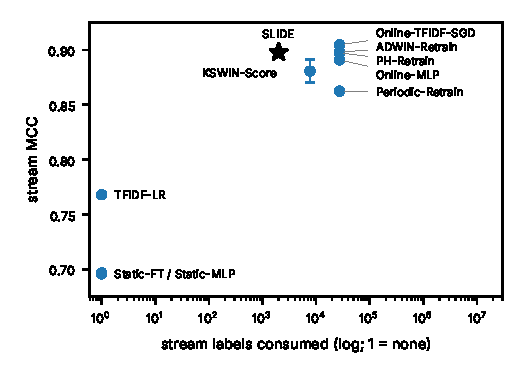
\includegraphics[width=0.62\linewidth]{figures/pareto.pdf}
\caption{Stream MCC against stream labels consumed (mean and 95\% CI over 10 realisations; static methods plotted at one label). Only the label-on-alarm methods lie between the static and the fully supervised clusters; KSWIN-Score buys 3.85 times more labels than SLIDE for a lower MCC. Static-FT and Static-MLP overlap at the bottom left.}
\label{fig:pareto}
\end{figure}

Figure~\ref{fig:pareto} places these results on the label-cost axis. KSWIN-Score uses the same purchase size as SLIDE but buys 7{,}700 labels and ends lower (0.881); Periodic retraining with all labels stays below both (0.862). Table~\ref{tab:stats} gives the paired tests. The Friedman test rejects equal performance across the ten methods ($\chi^2_F=81.91$, $p=6.8\times10^{-14}$); with a Nemenyi critical difference of 4.28 ranks, SLIDE (mean rank 3.3) is separated from TFIDF-LR (8.0) and the two static transformer detectors (9.7 and 9.3) but from no adaptive method. The realisation-level Wilcoxon tests are sharper. SLIDE wins all ten paired realisations against the three static detectors and against Periodic retraining, each at the smallest Holm-adjusted $p$-value the design allows (0.0176), and it loses all ten against Online-TFIDF-SGD at the same $p$-value. Against ADWIN-Retrain and PH-Retrain it wins five and six realisations ($p_{\mathrm{Holm}}=1$). Two comparisons sit near the threshold. SLIDE exceeds Online-MLP by 0.007 MCC in eight of ten realisations ($p_{\mathrm{Holm}}=0.039$) and KSWIN-Score by 0.017 in eight of ten, a difference that does not reach significance ($p_{\mathrm{Holm}}=0.059$) because KSWIN-Score varies four times more across realisations.

\begin{table}[t]
\centering
\caption{SLIDE versus each competitor. $\Delta$MCC: mean paired difference; wins out of 10 realisations; two-sided Wilcoxon signed-rank tests with Holm correction on realisation-level MCC and PR-AUC ($n=10$, primary) and on batch-level MCC ($n=1120$, descriptive); $r_{rb}$: rank-biserial effect size. Friedman $\chi^2_F=81.91$, $p=6.8\times10^{-14}$; Nemenyi CD$_{0.05}=4.28$.}
\label{tab:stats}
\scriptsize
\setlength{\tabcolsep}{2.5pt}
\begin{tabular}{@{}lrrrrrrrr@{}}
\toprule
Competitor & $\Delta$MCC & wins & $p_{\mathrm{Holm}}$ & $r_{rb}$ & $p^{\mathrm{PR}}_{\mathrm{Holm}}$ & $p^{\mathrm{batch}}_{\mathrm{Holm}}$ & $r^{\mathrm{batch}}_{rb}$ & rank \\
\midrule
TFIDF-LR & +0.130 & 10 & 0.0176 & +1.00 & 0.0176 & 9.8e-102 & +0.74 & 8.0 \\
Online-TFIDF-SGD & -0.007 & 0 & 0.0176 & -1.00 & 0.0176 & 1.2e-05 & -0.17 & 1.1 \\
Static-FT & +0.202 & 10 & 0.0176 & +1.00 & 0.0176 & 3.4e-162 & +0.95 & 9.7 \\
Static-MLP & +0.201 & 10 & 0.0176 & +1.00 & 0.0176 & 5.4e-151 & +0.97 & 9.3 \\
Online-MLP & +0.007 & 8 & 0.0391 & +0.89 & 1 & 0.014 & -0.11 & 5.1 \\
Periodic-Retrain & +0.035 & 10 & 0.0176 & +1.00 & 0.0176 & 0.45 & +0.05 & 6.8 \\
ADWIN-Retrain & -0.000 & 5 & 1 & -0.02 & 1 & 0.84 & +0.03 & 3.0 \\
PH-Retrain & +0.001 & 6 & 1 & +0.13 & 1 & 0.92 & -0.00 & 3.4 \\
KSWIN-Score & +0.017 & 8 & 0.0586 & +0.82 & 0.523 & 0.36 & +0.06 & 5.3 \\
\midrule
SLIDE (rank) & & & & & & & & 3.3 \\
\bottomrule
\end{tabular}
\end{table}


The batch-level tests are descriptive. Against the four retraining policies that react to time or to error (Periodic, ADWIN, Page--Hinkley and KSWIN-Score), the 1{,}120 paired batches show no difference ($p^{\mathrm{batch}}_{\mathrm{Holm}}\ge0.36$, $|r_{rb}|\le0.06$), so the stream-level gaps come from a few transition batches, not from a uniform offset. Against Online-MLP the two summaries disagree in sign ($r_{rb}=-0.11$ at batch level): Online-MLP wins slightly more individual batches while SLIDE has the higher pooled MCC, and we claim no advantage over Online-MLP beyond the realisation-level test.

\subsection{Alarm timing against equal-budget controls}\label{sec:controls}
Timing carries most of the label value. Table~\ref{tab:controls} holds the update rule fixed and varies only when the labels are bought. Spending the same 2{,}000 labels at random batches lowers MCC to 0.786 and segment-D MCC to 0.446 ($p_{\mathrm{Holm}}=0.0078$, the smallest value attainable over four rows), whereas buying them at the first moment that 500 messages of each new segment exist, which requires knowledge of the boundaries, gives 0.902, only 0.004 above SLIDE ($p_{\mathrm{Holm}}=0.059$). The score-based trigger behaves differently. With the SLIDE update, KSWIN on the score reaches 0.891 (7{,}550 labels): it is the best method on the paraphrase segment (0.932) and among the weakest adaptive ones on segment~D (0.766), and its spread across realisations ($\pm0.017$) is almost six times that of SLIDE. Part of the gap between SLIDE and KSWIN-Score in Table~\ref{tab:main} thus comes from the update rule; the remainder, at 3.8 times the label cost, is not significant ($p_{\mathrm{Holm}}=0.557$).

\begin{table}[t]
\centering
\caption{Controls that separate the timing of label purchases from the update rule (10 realisations). All rows except KSWIN-Score use the SLIDE update; Budget-Random buys four 500-label windows at random batches, Budget-Oracle buys them as soon as 500 messages of each new segment have arrived. $p_{\mathrm{Holm}}$: two-sided Wilcoxon test against SLIDE on realisation-level MCC, Holm-corrected over the four rows.}
\label{tab:controls}
\scriptsize
\setlength{\tabcolsep}{2.5pt}
\begin{tabular}{@{}lcccccr@{}}
\toprule
Method & MCC & MCC (D) & MCC (E) & Labels & $\Delta$ & $p_{\mathrm{Holm}}$ \\
\midrule
SLIDE & 0.898\,$\pm$\,0.003 & 0.825 & 0.894 & 2000 & -- & -- \\
KSWIN-Score & 0.881\,$\pm$\,0.012 & 0.765 & 0.832 & 7700 & -0.017 & 0.0586 \\
KSWIN-Score+SLIDE-update & 0.891\,$\pm$\,0.017 & 0.766 & 0.932 & 7550 & -0.007 & 0.557 \\
Budget-Random & 0.786\,$\pm$\,0.028 & 0.446 & 0.773 & 2000 & -0.112 & 0.00781 \\
Budget-Oracle & 0.902\,$\pm$\,0.003 & 0.822 & 0.899 & 2000 & +0.004 & 0.0586 \\
\bottomrule
\end{tabular}
\end{table}


\subsection{Behaviour at segment boundaries}\label{sec:boundaries}
Figure~\ref{fig:trajectory} shows where the gaps arise. All methods coincide on segment~A, and the static detectors fall to a batch MCC near 0.2 on the LLM segment~D. SLIDE raised exactly four alarms in each of the ten streams, one per boundary and none inside segment~A: at the first batch of segments B and D in every stream, and one batch after the B$\to$C and D$\to$E boundaries in eight of ten streams. The purchased labels arrive $D=2$ batches after the alarm, and the head is updated in that same batch; until then SLIDE scores with the old head, and the dip at C$\to$D in Fig.~\ref{fig:trajectory} spans those batches. ADWIN and Page--Hinkley watch the delayed error stream instead. They alarm on average 3.5 and 3.6 times per stream, retrain on the last 1{,}000 labels instead of 500 and keep receiving every later label, which explains why they match SLIDE on segment~D with 13.75 times more labels.

\begin{figure*}[t]
\centering
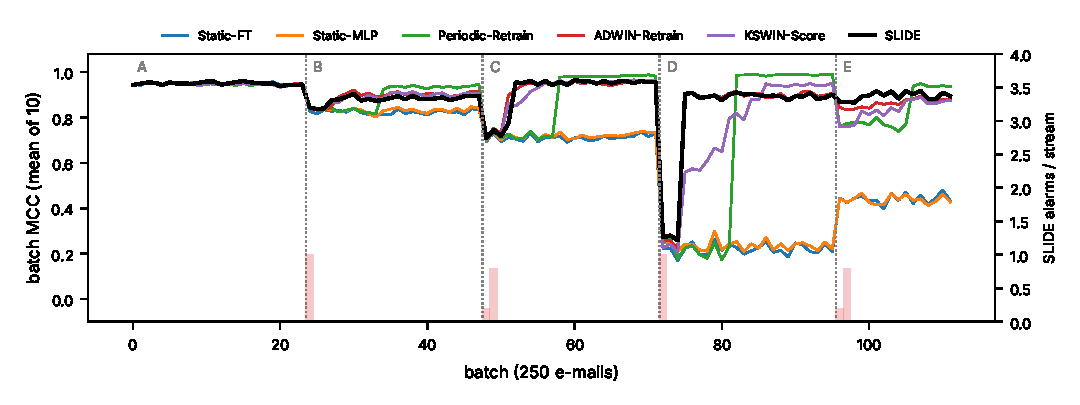
\includegraphics[width=0.95\linewidth]{figures/trajectory.pdf}
\caption{Batch MCC along the stream (mean over 10 realisations) and SLIDE alarms per batch (bars, right axis). Dotted lines mark segment boundaries.}
\label{fig:trajectory}
\end{figure*}

The two gates play distinct roles (Fig.~\ref{fig:swtrace}). At the 40 alarms the ratio $\widehat{SW}_1/\tau_\alpha$ had a median of 1.18 at A$\to$B, 1.57 at B$\to$C, 2.19 at C$\to$D and 1.33 at D$\to$E; the minimum KS $p$-value never exceeded $8.9\times10^{-5}$ and was below $10^{-7}$ at 36 of the 40 alarms. Over the 750 tests that did not alarm, the SW gate alone would never have fired, whereas the KS gate alone would have fired twelve times. KSWIN on the score stream, by comparison, triggered 15.4 refits per stream for four true changes.

\begin{figure}[t]
\centering
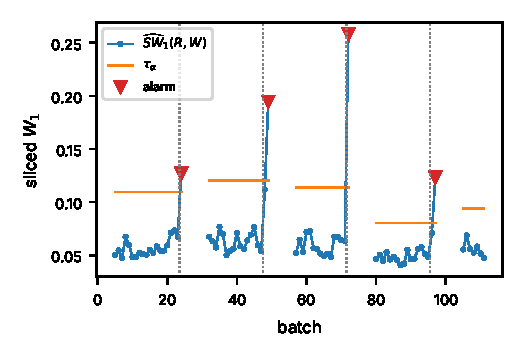
\includegraphics[width=0.62\linewidth]{figures/swtrace.pdf}
\caption{Sliced $W_1$ between reference and test window, calibrated threshold $\tau_\alpha$ and alarms for realisation 0. The threshold is re-estimated whenever the reference is rebuilt after an update; gaps mark batches without a test while the new reference and test window fill.}
\label{fig:swtrace}
\end{figure}

\begin{table}[t]
\centering
\caption{MCC per stream segment (mean over 10 realisations). Best value per column in bold.}
\label{tab:segments}
\scriptsize
\setlength{\tabcolsep}{3.5pt}
\begin{tabular}{@{}lccccc@{}}
\toprule
Method & A & B & C & D & E \\
\midrule
TFIDF-LR & \textbf{0.956} & 0.825 & 0.891 & 0.433 & 0.557 \\
Online-TFIDF-SGD & 0.925 & 0.869 & 0.920 & \textbf{0.892} & \textbf{0.897} \\
Static-FT & 0.948 & 0.824 & 0.711 & 0.221 & 0.442 \\
Static-MLP & 0.951 & 0.831 & 0.720 & 0.237 & 0.439 \\
Online-MLP & 0.946 & 0.889 & \textbf{0.924} & 0.768 & 0.895 \\
Periodic-Retrain & 0.947 & 0.892 & 0.867 & 0.711 & 0.831 \\
ADWIN-Retrain & 0.951 & 0.892 & 0.916 & 0.827 & 0.863 \\
PH-Retrain & 0.951 & \textbf{0.899} & 0.911 & 0.827 & 0.856 \\
KSWIN-Score & 0.946 & 0.888 & 0.910 & 0.765 & 0.832 \\
SLIDE & 0.950 & 0.879 & 0.915 & 0.825 & 0.894 \\
\bottomrule
\end{tabular}
\end{table}


Per-segment MCC (Table~\ref{tab:segments}) separates the two shift types. On the generator shift (D) SLIDE reaches 0.825, level with the error-triggered detectors (0.827) and behind Online-TFIDF-SGD (0.892). On the paraphrase campaign (E) it reaches 0.894, ahead of ADWIN (0.863) and Page--Hinkley (0.856) and level with Online-TFIDF-SGD (0.897) and Online-MLP (0.895). The ablation in Section~\ref{sec:ablation} does not attribute the segment-E advantage to any single term of the objective.

\subsection{Authorship slices}\label{sec:slices}
The style confound of Section~\ref{sec:audit} is visible in every transformer detector. Table~\ref{tab:slices} shows that SLIDE recovers 88.0\% of LLM-written phishing in segment~D and 93.7\% of paraphrased phishing in segment~E, whereas the static fine-tuned encoder detects 20.7\% and 36.5\%. SLIDE also flags 15.7\% of LLM-written \emph{legitimate} messages in segment~D, against 2.8\% of the human legitimate mail that sits in the same batches. Every transformer head shows the same pattern, with FPR on LLM-written legitimate mail between 6.8\% (Periodic retraining, at lower recall) and 27.0\% (Static-MLP). Online-TFIDF-SGD reaches comparable recall at 4.4\% FPR on that slice. Once it has seen every label, a word-level online model separates intent from style better than any frozen-encoder head here, and this is the largest gap in favour of a baseline that we observe.

\begin{table}[t]
\centering
\caption{Recall on malicious and FPR on legitimate messages by authorship inside segments D and E (mean over realisations; segment D contains no human-written malicious mail). ``llm'' = LLM-written, ``para'' = T1-paraphrased (malicious and the legitimate control).}
\label{tab:slices}
\scriptsize
\setlength{\tabcolsep}{2.5pt}
\begin{tabular}{@{}lccccc@{}}
\toprule
 & \multicolumn{2}{c}{Recall} & \multicolumn{3}{c}{FPR} \\
\cmidrule(lr){2-3}\cmidrule(lr){4-6}
Method & D:llm & E:para & D:llm & D:human & E:para \\
\midrule
TFIDF-LR & 0.602 & 0.670 & 0.517 & 0.080 & 0.494 \\
Online-TFIDF-SGD & 0.887 & 0.914 & 0.044 & 0.008 & 0.044 \\
Static-FT & 0.207 & 0.365 & 0.184 & 0.028 & 0.158 \\
Static-MLP & 0.272 & 0.418 & 0.270 & 0.044 & 0.252 \\
Online-MLP & 0.841 & 0.934 & 0.217 & 0.034 & 0.204 \\
Periodic-Retrain & 0.662 & 0.810 & 0.068 & 0.013 & 0.055 \\
ADWIN-Retrain & 0.875 & 0.901 & 0.135 & 0.028 & 0.168 \\
PH-Retrain & 0.876 & 0.892 & 0.137 & 0.028 & 0.165 \\
KSWIN-Score & 0.779 & 0.859 & 0.114 & 0.023 & 0.192 \\
SLIDE & 0.880 & 0.937 & 0.157 & 0.028 & 0.185 \\
\bottomrule
\end{tabular}
\end{table}


\subsection{Adversarial stress test}\label{sec:stress}
The stress pool (600 held-out phishing e-mails, Table~\ref{tab:pools}) is scored by each detector as it stands before the stream ($t_0$) and just before segment~E (pre-E), under each attack of Section~\ref{sec:threat}. The paraphraser met the attacker's constraint in most cases. The median MiniLM similarity of the rewrites was 0.912 and 96.6\% reached the 0.70 threshold within three attempts; the remaining 3.4\% keep their original text, as the threat model requires. The median word-level edit fraction was 0.58.

\begin{table*}[t]
\centering
\caption{Stress test on the held-out phishing pool: detection rate (recall at 0.5) before the stream ($t_0$) and at the D$\to$E boundary (pre-E), mean over 10 realisations.}
\label{tab:stress}
\scriptsize
\setlength{\tabcolsep}{2.5pt}
\resizebox{\textwidth}{!}{\begin{tabular}{@{}lcccccccccccccc@{}}
\toprule
 & \multicolumn{7}{c}{$t_0$ (warm-up model)} & \multicolumn{7}{c}{pre-E (after segments A--D)} \\
\cmidrule(lr){2-8}\cmidrule(lr){9-15}
Method & orig. & T1 & T2 .05 & T2 .10 & T2 .20 & T3 & T1$\circ$T2 & orig. & T1 & T2 .05 & T2 .10 & T2 .20 & T3 & T1$\circ$T2 \\
\midrule
TFIDF-LR & 0.712 & 0.645 & 0.705 & 0.687 & 0.698 & 0.448 & 0.650 & 0.712 & 0.645 & 0.705 & 0.687 & 0.698 & 0.448 & 0.650 \\
Online-TFIDF-SGD & 0.703 & 0.661 & 0.703 & 0.692 & 0.688 & 0.481 & 0.657 & 0.797 & 0.758 & 0.789 & 0.787 & 0.772 & 0.617 & 0.742 \\
Static-FT & 0.417 & 0.355 & 0.465 & 0.497 & 0.532 & 0.067 & 0.430 & 0.417 & 0.355 & 0.465 & 0.497 & 0.532 & 0.067 & 0.430 \\
Static-MLP & 0.462 & 0.407 & 0.509 & 0.527 & 0.556 & 0.103 & 0.480 & 0.462 & 0.407 & 0.509 & 0.527 & 0.556 & 0.103 & 0.480 \\
Online-MLP & 0.462 & 0.407 & 0.509 & 0.527 & 0.556 & 0.103 & 0.480 & 0.908 & 0.880 & 0.920 & 0.918 & 0.912 & 0.058 & 0.882 \\
Periodic-Retrain & 0.462 & 0.407 & 0.509 & 0.527 & 0.556 & 0.103 & 0.480 & 0.681 & 0.684 & 0.676 & 0.672 & 0.645 & 0.046 & 0.639 \\
ADWIN-Retrain & 0.462 & 0.407 & 0.509 & 0.527 & 0.556 & 0.103 & 0.480 & 0.938 & 0.897 & 0.948 & 0.937 & 0.900 & 0.099 & 0.874 \\
PH-Retrain & 0.462 & 0.407 & 0.509 & 0.527 & 0.556 & 0.103 & 0.480 & 0.938 & 0.897 & 0.948 & 0.937 & 0.900 & 0.099 & 0.874 \\
KSWIN-Score & 0.462 & 0.407 & 0.509 & 0.527 & 0.556 & 0.103 & 0.480 & 0.719 & 0.698 & 0.721 & 0.718 & 0.709 & 0.049 & 0.677 \\
SLIDE & 0.459 & 0.406 & 0.506 & 0.529 & 0.556 & 0.101 & 0.484 & 0.948 & 0.914 & 0.955 & 0.948 & 0.907 & 0.106 & 0.897 \\
\bottomrule
\end{tabular}}
\end{table*}


Table~\ref{tab:stress} supports three observations and one negative result. Paraphrase is the most effective content-preserving attack: T1 lowers SLIDE's detection rate from 0.948 to 0.914 at pre-E and from 0.459 to 0.406 at $t_0$. Character perturbation alone is weak. At $t_0$ higher rates even \emph{raise} detection for every transformer head (0.459 to 0.556 for SLIDE); homoglyphs and zero-width characters are rare in legitimate mail, so they act as a malicious signal. After adaptation SLIDE has the highest detection rate in five of the seven pre-E columns, with 0.914 under T1 and 0.897 under T1$\circ$T2 against 0.897 and 0.874 for ADWIN-Retrain; Online-MLP is ahead at $\epsilon_{\mathrm{char}}=0.20$ (0.912 against 0.907). Benign padding is the negative result. A 400-character legitimate prefix lowers the detection rate of every transformer-based method to 0.046--0.106 at both time points, whereas the TF-IDF models, which read the whole message, keep 0.45--0.62.

\begin{table}[t]
\centering
\caption{Left: displacement $\lVert\Phi(x')-\Phi(x)\rVert_2$ caused by each attack on the 600 stress e-mails (median, 10th--90th percentile; rel.: median ratio to $\lVert\Phi(x)\rVert_2$). Right: fraction of the stress e-mails that the warm-up head classifies correctly \emph{and} certifies by Proposition~\ref{prop:cert} at radius $\epsilon$, for a plain head and for a head trained with the adversarial term ($\lambda_a{=}0.5$, $\epsilon{=}1$).}
\label{tab:cert}
\scriptsize
\setlength{\tabcolsep}{2.5pt}
\begin{tabular}{@{}lrr@{\hspace{8pt}}lrr@{}}
\toprule
Attack & median (q10--q90) & rel. & radius $\epsilon$ & plain & adv. \\
\midrule
T1 paraphrase & 11.1 (5.4--21.9) & 0.40 & 0.25 & 0.438 & 0.435 \\
T2, $\epsilon_{\mathrm{char}}{=}0.05$ & 5.7 (2.6--10.8) & 0.21 & 0.5 & 0.415 & 0.427 \\
T2, $\epsilon_{\mathrm{char}}{=}0.10$ & 9.1 (4.8--16.0) & 0.33 & 1 & 0.358 & 0.370 \\
T2, $\epsilon_{\mathrm{char}}{=}0.20$ & 14.6 (7.7--24.5) & 0.53 & 2 & 0.167 & 0.203 \\
T3 padding & 30.8 (17.1--47.6) & 1.03 & $L_m$ & 6.04 & 5.45 \\
T1$\circ$T2 (0.10) & 14.6 (9.4--23.9) & 0.50 & recall & 0.460 & 0.465 \\
\bottomrule
\end{tabular}
\end{table}


Table~\ref{tab:cert} explains why the certificate of Proposition~\ref{prop:cert} cannot cover these attacks. The median displacement in $\Phi$ ranges from 5.7 (T2 at 0.05) through 11.1 (T1) to 30.8 (T3) standard-deviation units, i.e.\ 21--103\% of the norm of the original representation, while the head certifies at most 43.8\% of the stress e-mails at radius 0.25 and 20.3\% at radius 2. The adversarial term lowers the Lipschitz bound $L_m$ from 6.04 to 5.45 and raises the certified fraction at radii 0.5--2 (from 0.167 to 0.203 at $\epsilon=2$) at unchanged recall. That gain is real but an order of magnitude too small for text-level attacks; the observed robustness to T1 after adaptation comes from the labelled campaign data, not from the certificate.

\subsection{Ablation}\label{sec:ablation}
Table~\ref{tab:ablation} removes one component at a time. Two components carry the result. Without adaptation the detector stays at the static level (0.698). A drift test on the score alone raises only 1.5 alarms per stream (750 labels) and ends at 0.838; the projections of $\Phi$ are what make the shift visible, and the projections-only test reproduces SLIDE exactly. Of the objective's terms only the adversarial one has a measurable effect, 0.003 MCC consistent across the ten realisations ($p_{\mathrm{Holm}}=0.0176$). Removing the proximal term or the replay buffer changes nothing measurable, and neither does dropping the surprisal features $\psi$ ($|\Delta|\le0.002$, $p_{\mathrm{Holm}}\ge0.22$). Either gate alone still yields about four alarms per stream (2{,}000 labels without the KS gate, 2{,}100 without the SW gate); on this stream the conjunction mainly suppresses the occasional extra alarm.

\begin{table}[t]
\centering
\caption{Ablation over 10 realisations. $\Delta$: change of mean MCC relative to full SLIDE; $p$: Holm-corrected two-sided Wilcoxon test against full SLIDE on realisation-level MCC.}
\label{tab:ablation}
\scriptsize
\setlength{\tabcolsep}{2.5pt}
\begin{tabular}{@{}lccccrr@{}}
\toprule
Variant & MCC & PR-AUC & MCC (E) & Labels & $\Delta$ & $p_{\mathrm{Holm}}$ \\
\midrule
SLIDE & 0.898\,$\pm$\,0.003 & 0.977 & 0.894 & 2000 & -- & -- \\
SLIDE w/o adversarial term & 0.895\,$\pm$\,0.002 & 0.975 & 0.890 & 2000 & -0.003 & 0.0176 \\
SLIDE w/o replay & 0.900\,$\pm$\,0.003 & 0.977 & 0.890 & 2000 & +0.002 & 0.527 \\
SLIDE w/o proximal term & 0.899\,$\pm$\,0.003 & 0.977 & 0.894 & 2000 & +0.001 & 0.223 \\
SLIDE w/o surprisal $\psi$ & 0.898\,$\pm$\,0.004 & 0.976 & 0.895 & 2000 & -0.000 & 1 \\
SLIDE w/o KS gate & 0.898\,$\pm$\,0.003 & 0.977 & 0.894 & 2000 & +0.000 & 1 \\
SLIDE w/o SW gate & 0.899\,$\pm$\,0.003 & 0.976 & 0.900 & 2100 & +0.001 & 0.594 \\
SLIDE score-only test & 0.838\,$\pm$\,0.010 & 0.950 & 0.843 & 750 & -0.060 & 0.0176 \\
SLIDE projections-only test & 0.898\,$\pm$\,0.003 & 0.977 & 0.894 & 2000 & +0.000 & 1 \\
SLIDE w/o adaptation & 0.698\,$\pm$\,0.002 & 0.898 & 0.443 & 0 & -0.200 & 0.0176 \\
\bottomrule
\end{tabular}
\end{table}


\subsection{Sensitivity}\label{sec:sens}
SLIDE is insensitive to its test and robustness settings within the ranges of Table~\ref{tab:sens}. Over five realisations, MCC stays between 0.895 and 0.899 for $\epsilon\in[0.25,4]$, $\alpha\in[0.001,0.05]$ and $K\in\{16,256\}$, against 0.896 at the default; only $\alpha=0.05$ (2{,}200 labels) and $K=256$ (2{,}100) buy an extra window. The purchase size is the one lever with a visible trade-off. At $n_\ell=250$ SLIDE spends 1{,}000 labels and loses 0.008 MCC overall and 0.028 on the paraphrase segment; at $n_\ell=1000$ it spends 4{,}000 labels and gains 0.004 overall and 0.024 on that segment.

\begin{table}[t]
\centering
\caption{Sensitivity of SLIDE (5 realisations; default: $\epsilon=1$, $\alpha=0.01$, $n_\ell=500$, $K=64$; first row shows the default on the same 5 realisations).}
\label{tab:sens}
\scriptsize
\begin{tabular}{@{}lcccr@{}}
\toprule
Setting & MCC & MCC (E) & FPR & Labels \\
\midrule
default & 0.896 & 0.890 & 0.042 & 2000 \\
$\epsilon$=0.25 & 0.895 & 0.891 & 0.043 & 2000 \\
$\epsilon$=0.5 & 0.895 & 0.892 & 0.043 & 2000 \\
$\epsilon$=2.0 & 0.899 & 0.892 & 0.040 & 2000 \\
$\epsilon$=4.0 & 0.895 & 0.876 & 0.041 & 2000 \\
$\alpha$=0.001 & 0.895 & 0.888 & 0.042 & 2000 \\
$\alpha$=0.05 & 0.899 & 0.898 & 0.042 & 2200 \\
$n_\ell$=250 & 0.888 & 0.862 & 0.045 & 1000 \\
$n_\ell$=1000 & 0.900 & 0.914 & 0.039 & 4000 \\
$K$=16 & 0.897 & 0.893 & 0.042 & 2000 \\
$K$=256 & 0.897 & 0.893 & 0.042 & 2100 \\
\bottomrule
\end{tabular}
\end{table}


\subsection{Computational cost}\label{sec:cost}
The drift machinery is cheap; the transformers are not. Table~\ref{tab:latency} shows that one drift test costs 77\,ms per 250-message batch in isolation (0.31\,ms per e-mail) and 174\,ms inside the stream, where the reference and window buffers are also maintained; the encoder pass costs 27\,ms per e-mail on four threads and the surprisal model 72\,ms. A SLIDE update with PGD and replay takes 2.3\,s in isolation and 3.8\,s on average inside the stream, four times per stream. The persistent state at full reservoir capacity occupies 6.8\,MB. Since the ablation shows no benefit from $\psi$, dropping the surprisal model would cut the per-message cost by roughly 70\% on this stream.

\begin{table}[t]
\centering
\caption{Measured cost of each SLIDE component on one Intel Xeon Processor @ 2.10GHz (4 cores, no GPU). Transformer timings use batches of 32 e-mails of at most 128 tokens.}
\label{tab:latency}
\scriptsize
\setlength{\tabcolsep}{3pt}
\begin{tabular}{@{}>{\raggedright\arraybackslash}p{7cm}>{\raggedright\arraybackslash}p{6cm}@{}}
\toprule
Component & Cost \\
\midrule
DistilRoBERTa pass $\phi$ (1 / 4 threads) & 101.4 / 27.1 ms per e-mail \\
distilgpt2 surprisal $\psi$ (1 / 4 threads) & 240.5 / 71.6 ms per e-mail \\
Head $h_\theta$ scoring & 5.8 $\mu$s per e-mail \\
Drift test, isolated ($n_R{=}1000$, $n_W{=}500$, $K{=}64$) & 77.3 ms per batch (0.31 ms per e-mail) \\
Drift test, inside the stream & 173.8 ms per batch \\
Reference rebuild and calibration ($B{=}100$) & 0.91 s per alarm \\
Head update, plain CE / $\mathcal{L}_{\mathrm{total}}$ & 0.28 / 2.26 s per update \\
Head update inside the stream (mean) & 3.77 s per update \\
TF-IDF + LR scoring (reference) & 0.49 ms per e-mail \\
Parameters: encoder / LM / head & 82.1M / 81.9M / 198k \\
State at capacity: reservoir (2 classes $\times$ 1{,}000 $\times$ 772 float32) / reference / projections & 5.89 / 0.50 / 0.38 MB \\
\bottomrule
\end{tabular}
\end{table}


\section{Discussion}\label{sec:discussion}

\subsection{What the label budget buys}
The central trade-off is labels against accuracy. On this stream a fully supervised policy turns 27{,}500 labels into at most 0.007 MCC over SLIDE; equivalently, SLIDE retains 99.2\% of the best supervised MCC with 2{,}000 labels and equals the supervised, error-triggered retraining of its own head. Whether that is the right operating point depends on the price of a verified label. An analyst who must open and adjudicate every message cannot sustain full supervision at gateway volume, and the delayed-label baselines in Table~\ref{tab:main} are an upper reference rather than a deployable alternative. Where labels are cheap, for instance from user reports of a mature organisation, Online-TFIDF-SGD is a strong and inexpensive choice: it was the most accurate method overall and had the lowest false-positive rate on LLM-written legitimate mail.

The ablation and the controls narrow the claim. What SLIDE contributes is \emph{when} it buys labels, and that depends on \emph{where} it looks. At an equal budget, random purchase times cost 0.112 MCC and boundary-aware oracle times gain only 0.004 (Table~\ref{tab:controls}). A KS test on the detector score misses most changes (1.5 alarms for four shifts), and KSWIN on the same score raises 15.4 alarms; projecting $\Phi$ onto random directions exposes shifts that the score hides, because the head maps the new region onto confident but wrong scores. The robust objective matters less than its design suggests. Only the adversarial term has a measurable effect (0.003 MCC); the proximal term and replay show none on this stream, where every update warm-starts from the previous head. A score-triggered policy with the same update comes within 0.007 MCC of SLIDE, but at 3.8 times the label cost and with six times the spread across realisations.

\subsection{Deployment considerations}
SLIDE fits a gateway as an asynchronous side-car. Scoring needs one encoder pass per message while the drift test runs once per batch on cached vectors; an alarm becomes a labelling ticket for the last 500 messages, and the update itself takes seconds on a CPU. The surprisal model contributed nothing measurable here and accounts for about 70\% of the inference cost, so a deployment should drop it unless its own data show otherwise. Two operating rules follow from Section~\ref{sec:results}. The reference must be rebuilt only from post-update traffic, or the test compares the new head's regime with the old one and re-alarms. The purchase window must also be long enough to contain the new campaign; at $n_\ell=250$ the paraphrase segment lost 0.028 MCC.

\subsection{Threats to validity}\label{sec:validity}
\paragraph{Construct validity} The human corpora label spam and phishing together as \emph{malicious}; our detector therefore learns unsolicited bulk mail as well as credential phishing, and the human-written portion of the benchmark is not a pure phishing benchmark. The LLM segments, on the other hand, contain phishing only. The authorship probe (0.9996 macro-F1) shows that LLM-written mail is trivially separable from human mail by style, and the 6.8--27.0\% FPR of the transformer heads on LLM-written legitimate messages indicates that part of what they learn in segment~D is style rather than intent. We report this slice instead of hiding it in the stream average. A stream in which legitimate senders also adopt LLM writing would make this confound more costly.

\paragraph{Internal validity} All hyper-parameters were fixed before the stream runs, and every baseline shares SLIDE's representation and head, so the comparison isolates the policy. The encoder was fine-tuned on warm-up data drawn from the same three human corpora as segment~A, so segment~A is close to in-distribution for $\phi$ and the stream tests generalisation mainly from segment~B onward. The fully supervised baselines are not budget-matched: they receive every label, and only the controls of Table~\ref{tab:controls} compare policies at an equal label count. The baselines are also trained with plain cross-entropy, so part of any gap to them may come from the update rule rather than from the trigger, which the KSWIN-Score+SLIDE-update control measures directly. The baseline detectors use fixed, untuned settings (ADWIN $\delta=0.002$; Page--Hinkley threshold 50 with 200 warm-up observations; KSWIN $\alpha=0.005$ with window 500 and statistic size 150), not values selected on the stream; a tuned ADWIN or KSWIN might narrow or widen the gaps. Ten realisations bound the strength of the realisation-level Wilcoxon tests at an adjusted $p$ of 0.0176, and the batch-level tests treat dependent batches as pairs, so we read them as descriptive.

\paragraph{External validity} The stream is a controlled composition of public corpora with abrupt boundaries, not a recording of one organisation's traffic. Abrupt boundaries favour any window-based test, and each boundary also changes the source corpus, so the shift SLIDE detects mixes campaign change with corpus style. Neither gradual or recurring drift nor label noise was studied. The LLM corpora were generated with OpenAI models only, and the paraphrase campaign uses a single T5 paraphraser; a stronger generator--critic attacker \cite{qi2025} that queries the detector would likely do better than T1. Real drift with an unchanged input marginal is invisible to SLIDE and to every label-free test (Proposition~\ref{prop:sw}).

\paragraph{The padding attack} Prepending 400 characters of legitimate text defeated every transformer detector at every time point (Table~\ref{tab:stress}). The cause is structural: with a 128-token window the lure is pushed out of what $\phi$ and $\psi$ read. Segment-wise encoding with max-pooling over segments would close this specific gap, and so would a cheap whole-message model run in parallel; the TF-IDF results suggest that the second option is effective, and we leave its integration to future work.

\section{Conclusion}\label{sec:conclusion}

LLM-written phishing turns a static detection problem into a streaming one. SLIDE treats it that way: a label-free sliced two-gate test on transformer representations decides when to buy labels, and a four-term robust objective decides how to use them. On a 28{,}000-message public stream that moves from human corpora to two LLM corpora and a paraphrase campaign, the test detected all 40 segment changes within one batch without a false alarm. With 2{,}000 labels SLIDE reached an MCC of 0.898, against 0.897--0.905 for the best detectors that consumed all 27{,}500 labels and 0.696--0.768 for detectors that never adapt. The value lies in the timing of the purchases: the same budget spent at random times lost 0.112 MCC, and oracle timing gained only 0.004. Random projections of the representation make that timing possible; the same test on the detector score alone lost 0.060 MCC. Of the four loss terms only the adversarial one improved accuracy measurably.

Two findings bound the result. Transformer heads, SLIDE included, confound LLM style with malicious intent and flag 6.8--27.0\% of LLM-written legitimate mail, and a 400-character benign prefix defeats every 128-token transformer detector we tested. Future work should pair the drift-adaptive transformer with a whole-message model and evaluate the policy on gradual and recurring drift in an operational stream; adaptive attackers who query the deployed detector belong in the next version of the threat model.


\bibliographystyle{IEEEtran}
\bibliography{refs}

\end{document}
